\documentclass[a4paper, 50pt, twoside]{article}
\usepackage[italian]{babel}
\usepackage[a4paper, top=2cm, bottom=2cm, left=3cm, right=3cm]{geometry}
\usepackage{graphicx}
\graphicspath{{immagini/}}
\usepackage{chngcntr}
\counterwithin{figure}{section}
\usepackage{braket}
\usepackage{amsmath}
\usepackage{fancyhdr}
\usepackage{xcolor}
\pagestyle{fancy}
\lfoot{EasyVersity}

\begin{document}


\title{EasyVersity}
\date{Settembre, 2019}
\author{Tomassini Danilo \\ Simone Cappella \\ Luca Mannini \\ \\ Ingegneria Informatica e dell'Automazione}
\maketitle
\vspace*{\fill}
\begin{figure}[h!]
	\centering
	
\includegraphics[width=\linewidth]{copertina4.jpg}
	\label {fig::copertina}
\end{figure}
\vspace*{\fill}

\newpage
\tableofcontents{}

\newpage
\section{Obbiettivi}
EasyVersity rappresenta uno strumento di supporto per lo studente.

Permette di gestire:
\begin{itemize}
\item \textbf{Orario:} salva l'orario delle lezioni nella tua applicazione per consultarlo quando vuoi.
\item \textbf{Archivio appunti locale:} da la possibilità di salvare appunti raggruppandoli per materia, indicando titolo e data si può contestualizzare al meglio l'appunto in questione.
\item \textbf{Condivisione appunti:} rende possibile la condivisione ed il download degli appunti.
\item \textbf{Impostazioni:} da qui si possono cambiare informazioni come username e password, eprendere visione di info "about us".
\end{itemize}

\section{Funzionalità}
All'avvio dell'applicazione va effettuato il login o la registrazione.
\begin{figure}[!h]
	\centering
	{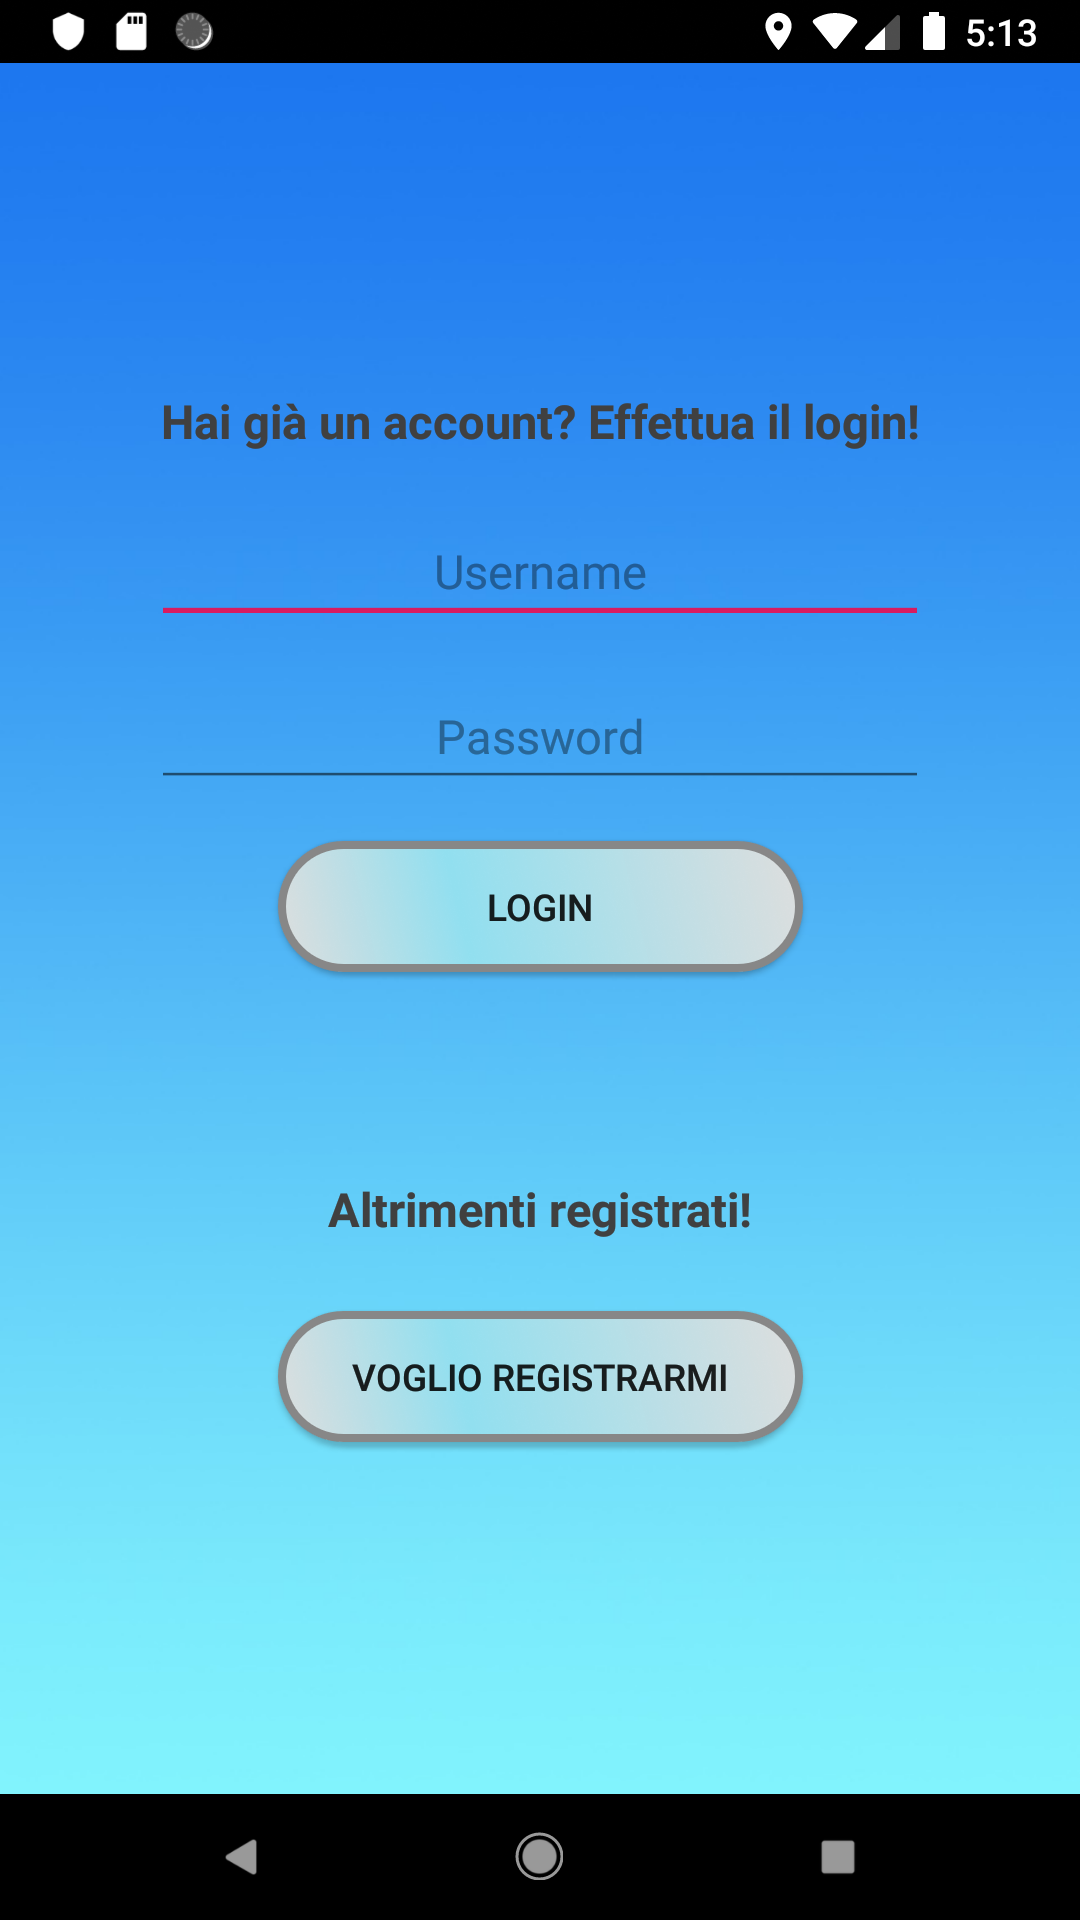
\includegraphics[width=.30\textwidth]{login}} \quad
	{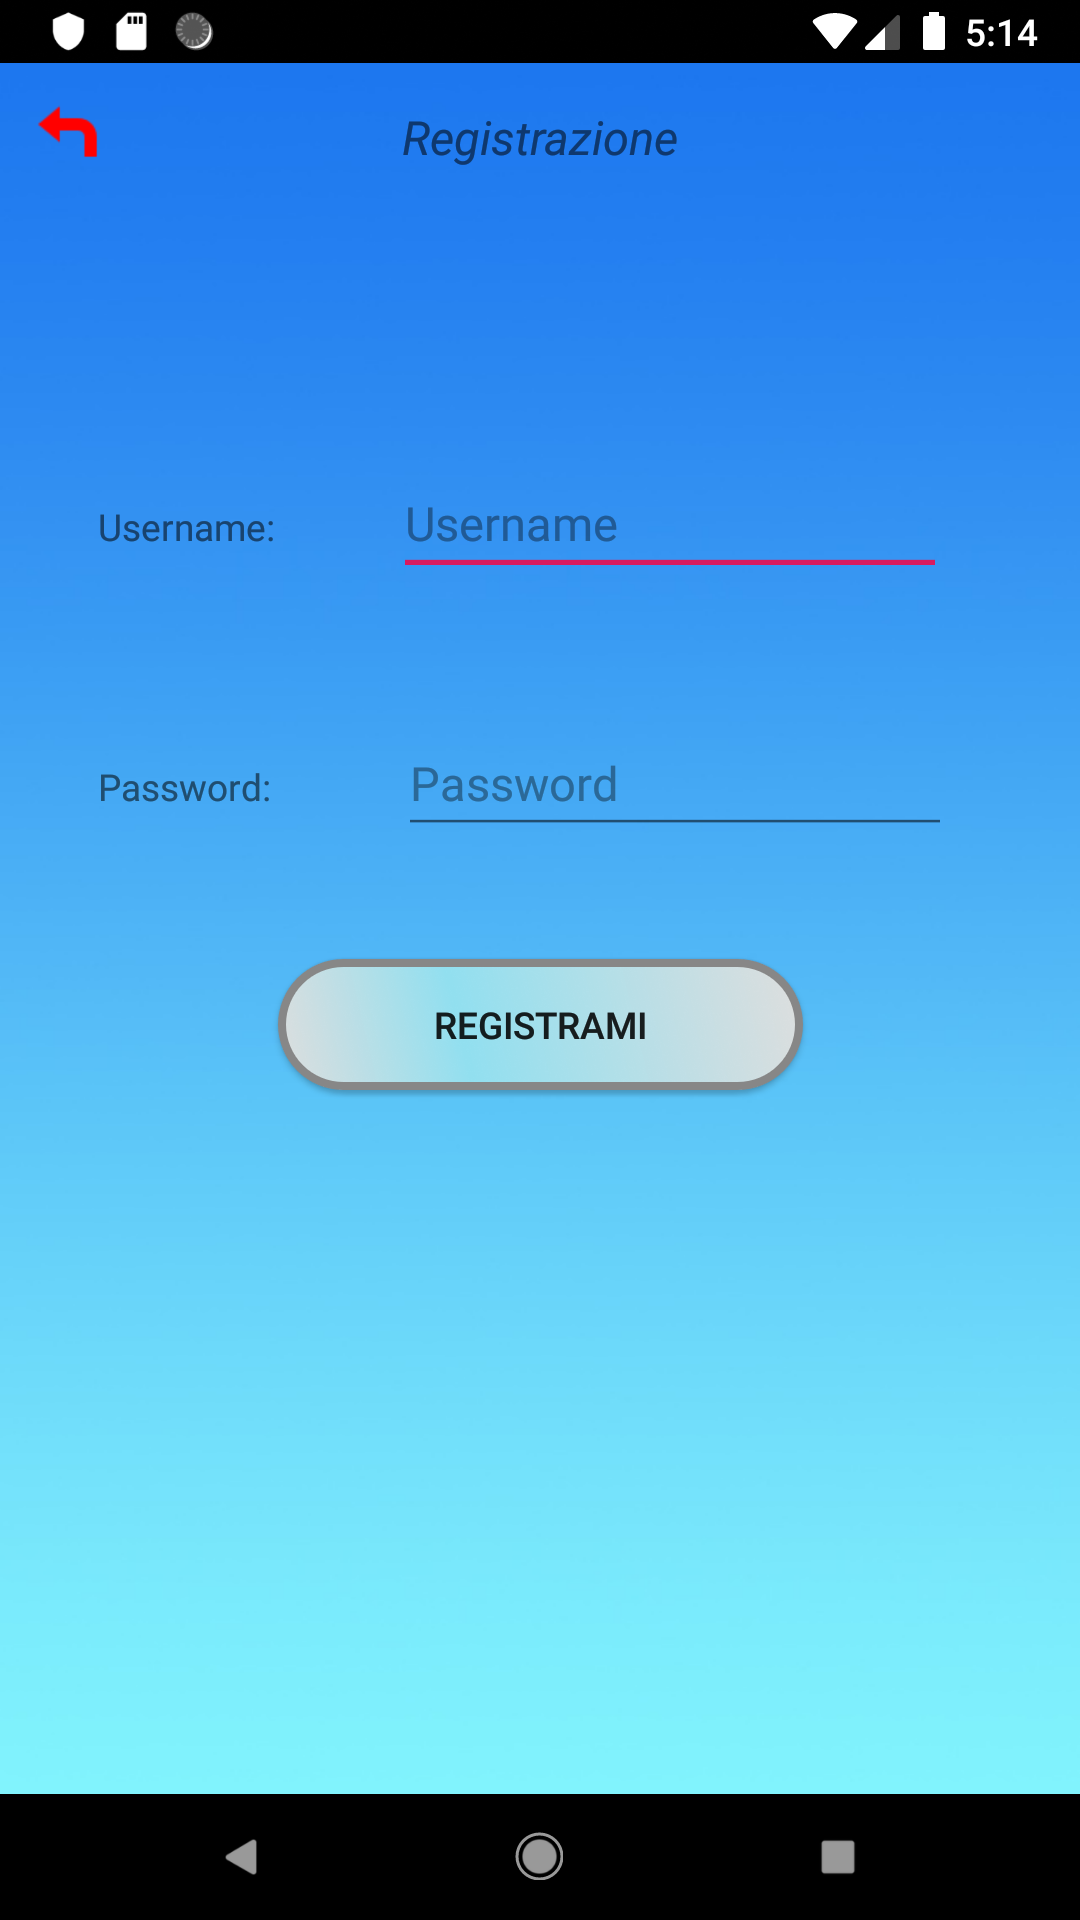
\includegraphics[width=.30\textwidth]{registrazione}} \quad
	{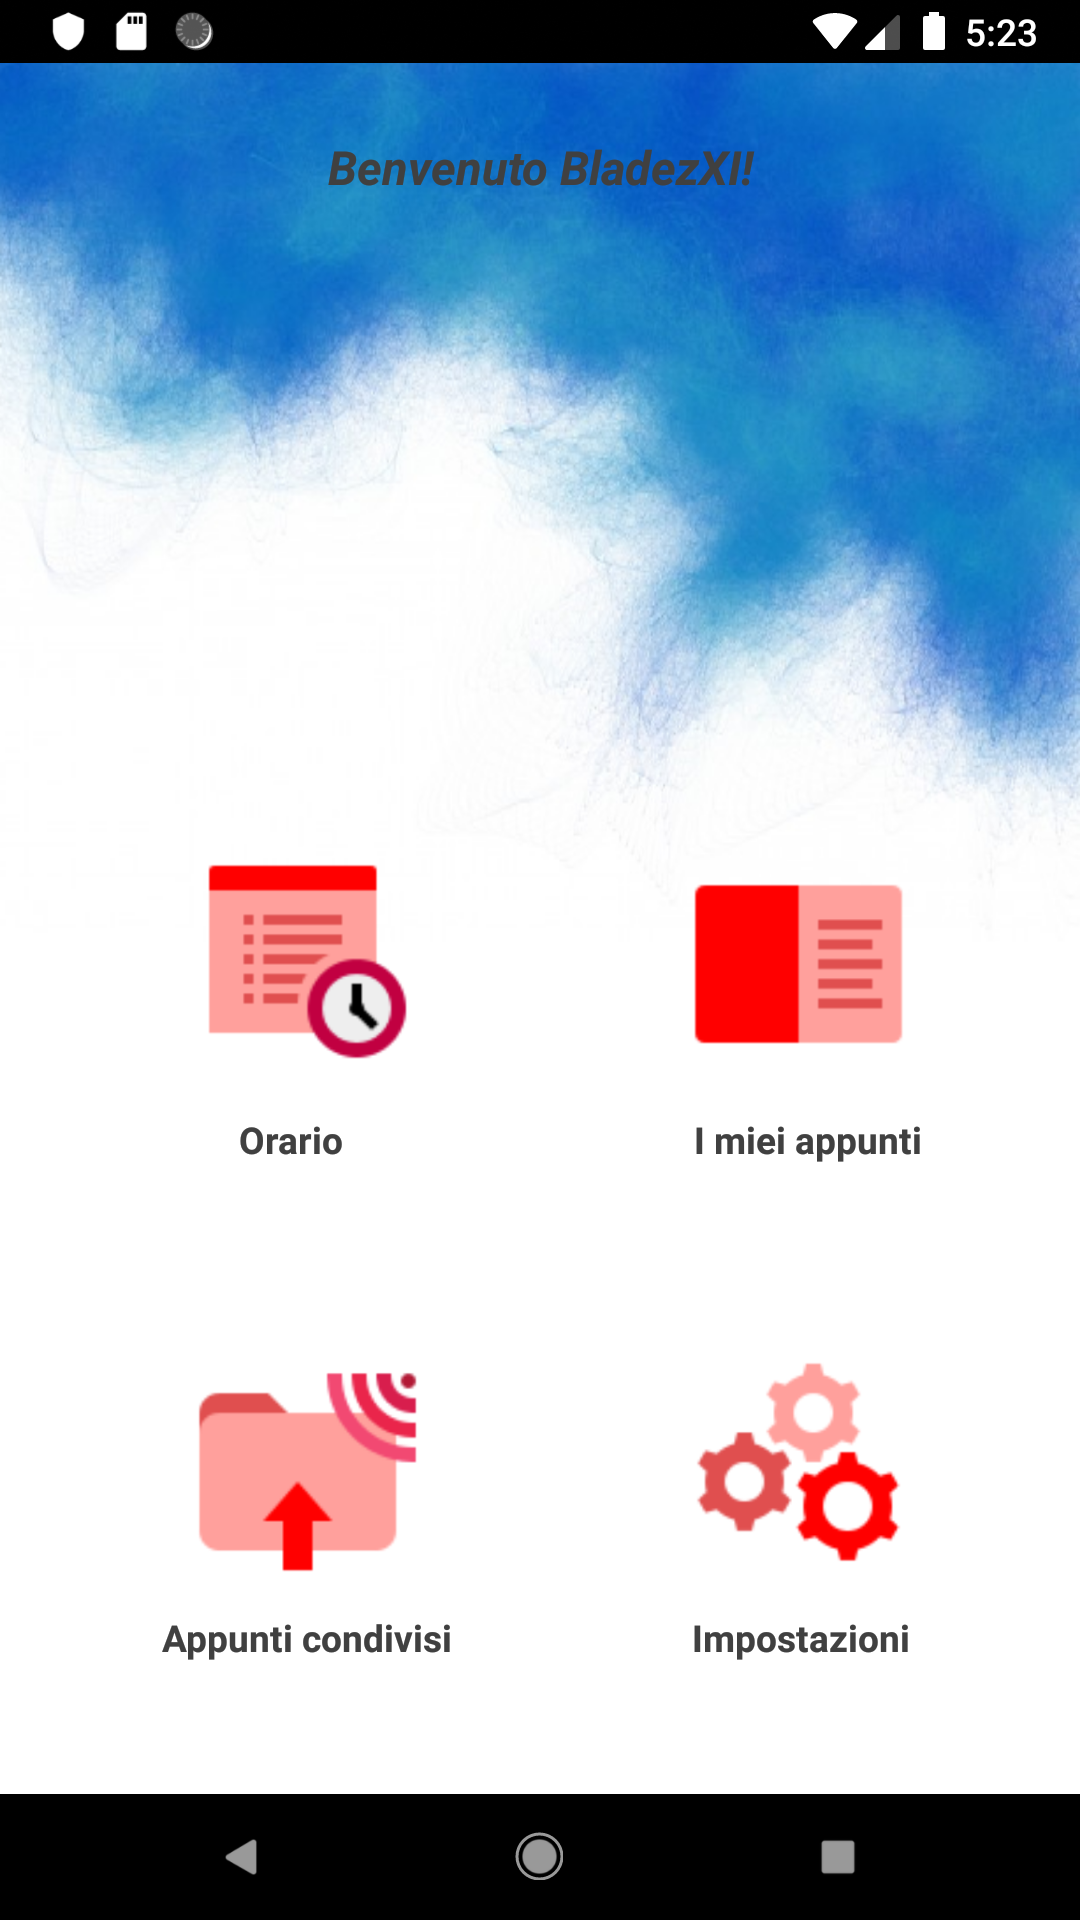
\includegraphics[width=.30\textwidth]{menu}}
	\caption{\small Schermata Login, Registrazione e Menu principale.}
\end{figure}

Una volta effettuato il login si può accedere al menù principale che prevede 4 scelte:
\begin{itemize}
\item \textbf{Orario.}
\item \textbf{I miei appunti.}
\item \textbf{Appunti condivisi.}
\item \textbf{Impostazioni.}
\end{itemize}

\newpage
\subsection{Orario}
Aperto l'orario ci si trova di fronte alla tabella relativa al giorno corrente; con la bottom navbar si può scegliere il giorno su cui andare ad agire.
Premendo nel campo \textbf{materia}, relativo all'ora di interesse si può inserire la materia in tabella, si accede, infatti, ad una lista predefinita di materie (questa può essere estesa scegliendo di inserirne una manualmente con il bottone "altro"). Scelta la materia viene visualizzata una finestra di dialogo che permette di inserire l'aula in cui si svolgerà la lezione e la durata della stessa.
\begin{figure}[!h]
	\centering
	{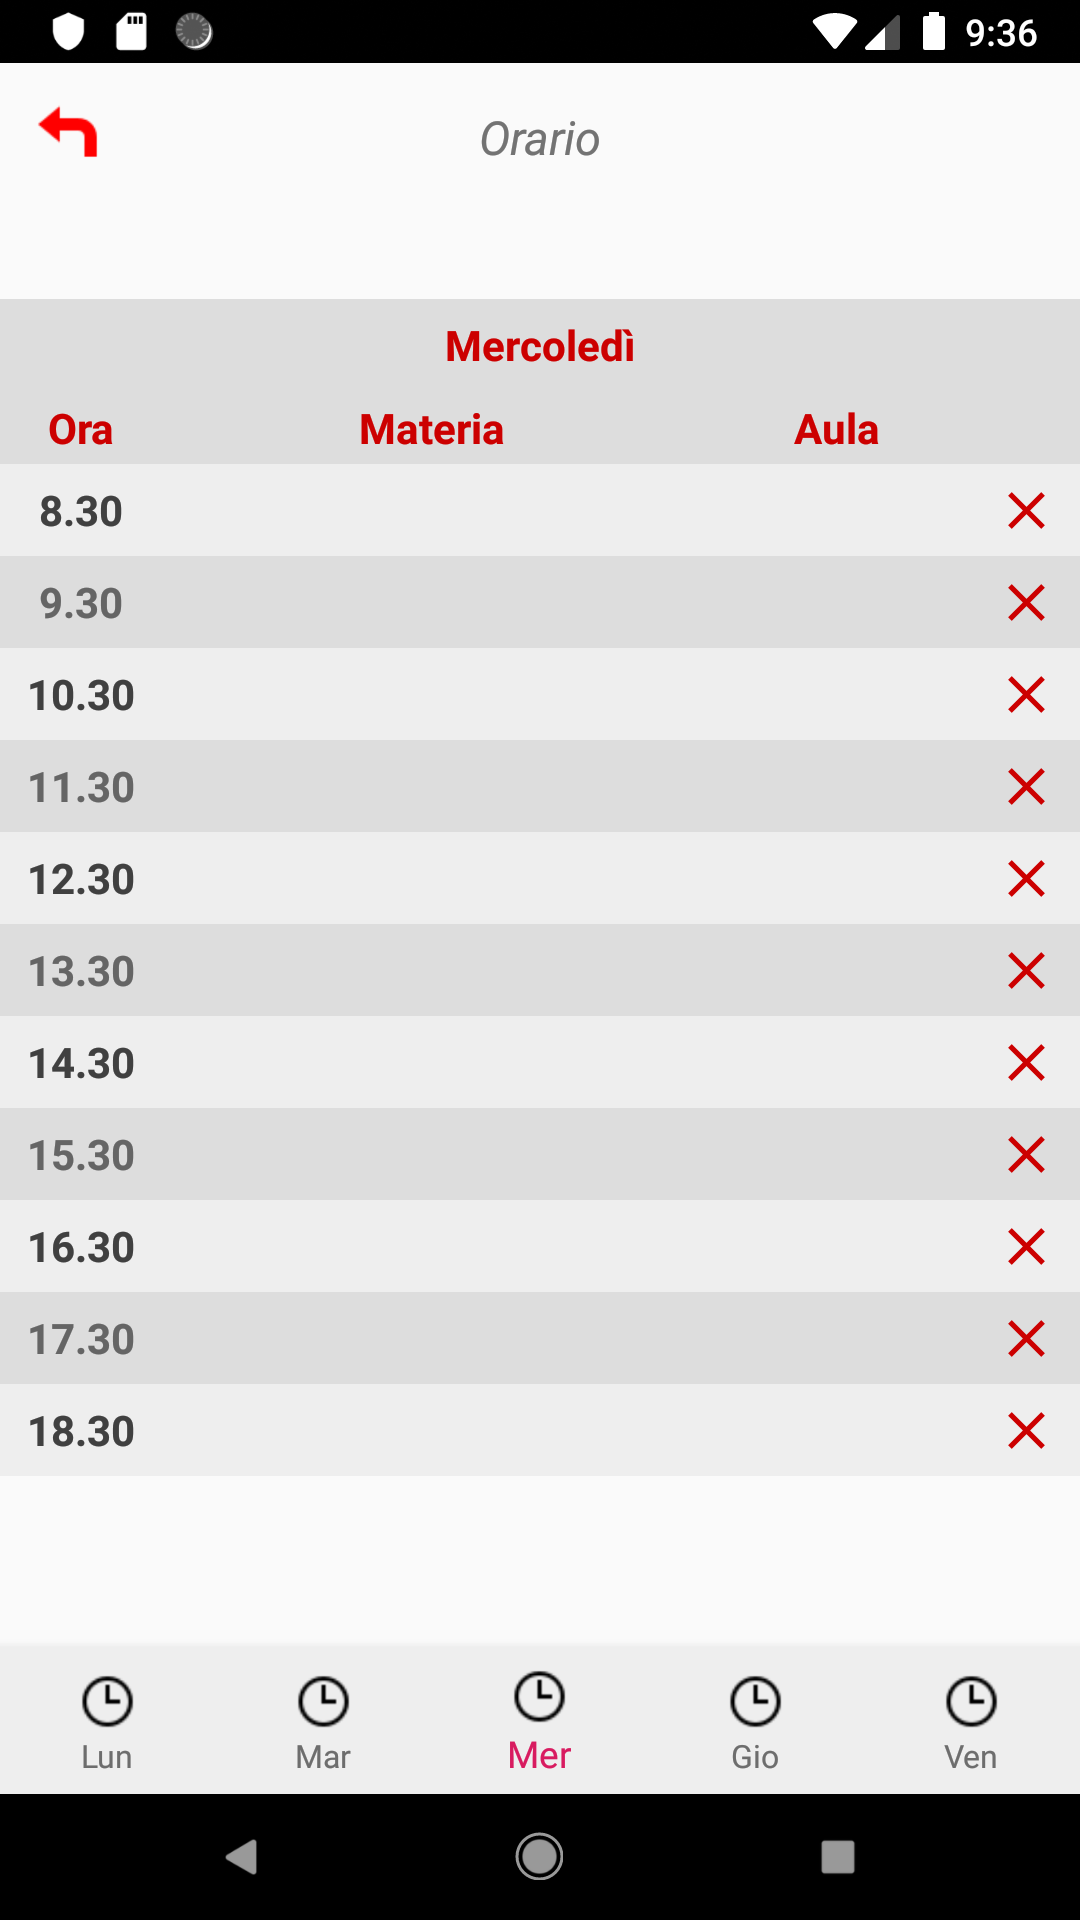
\includegraphics[width=.30\textwidth]{orario}} \quad
	{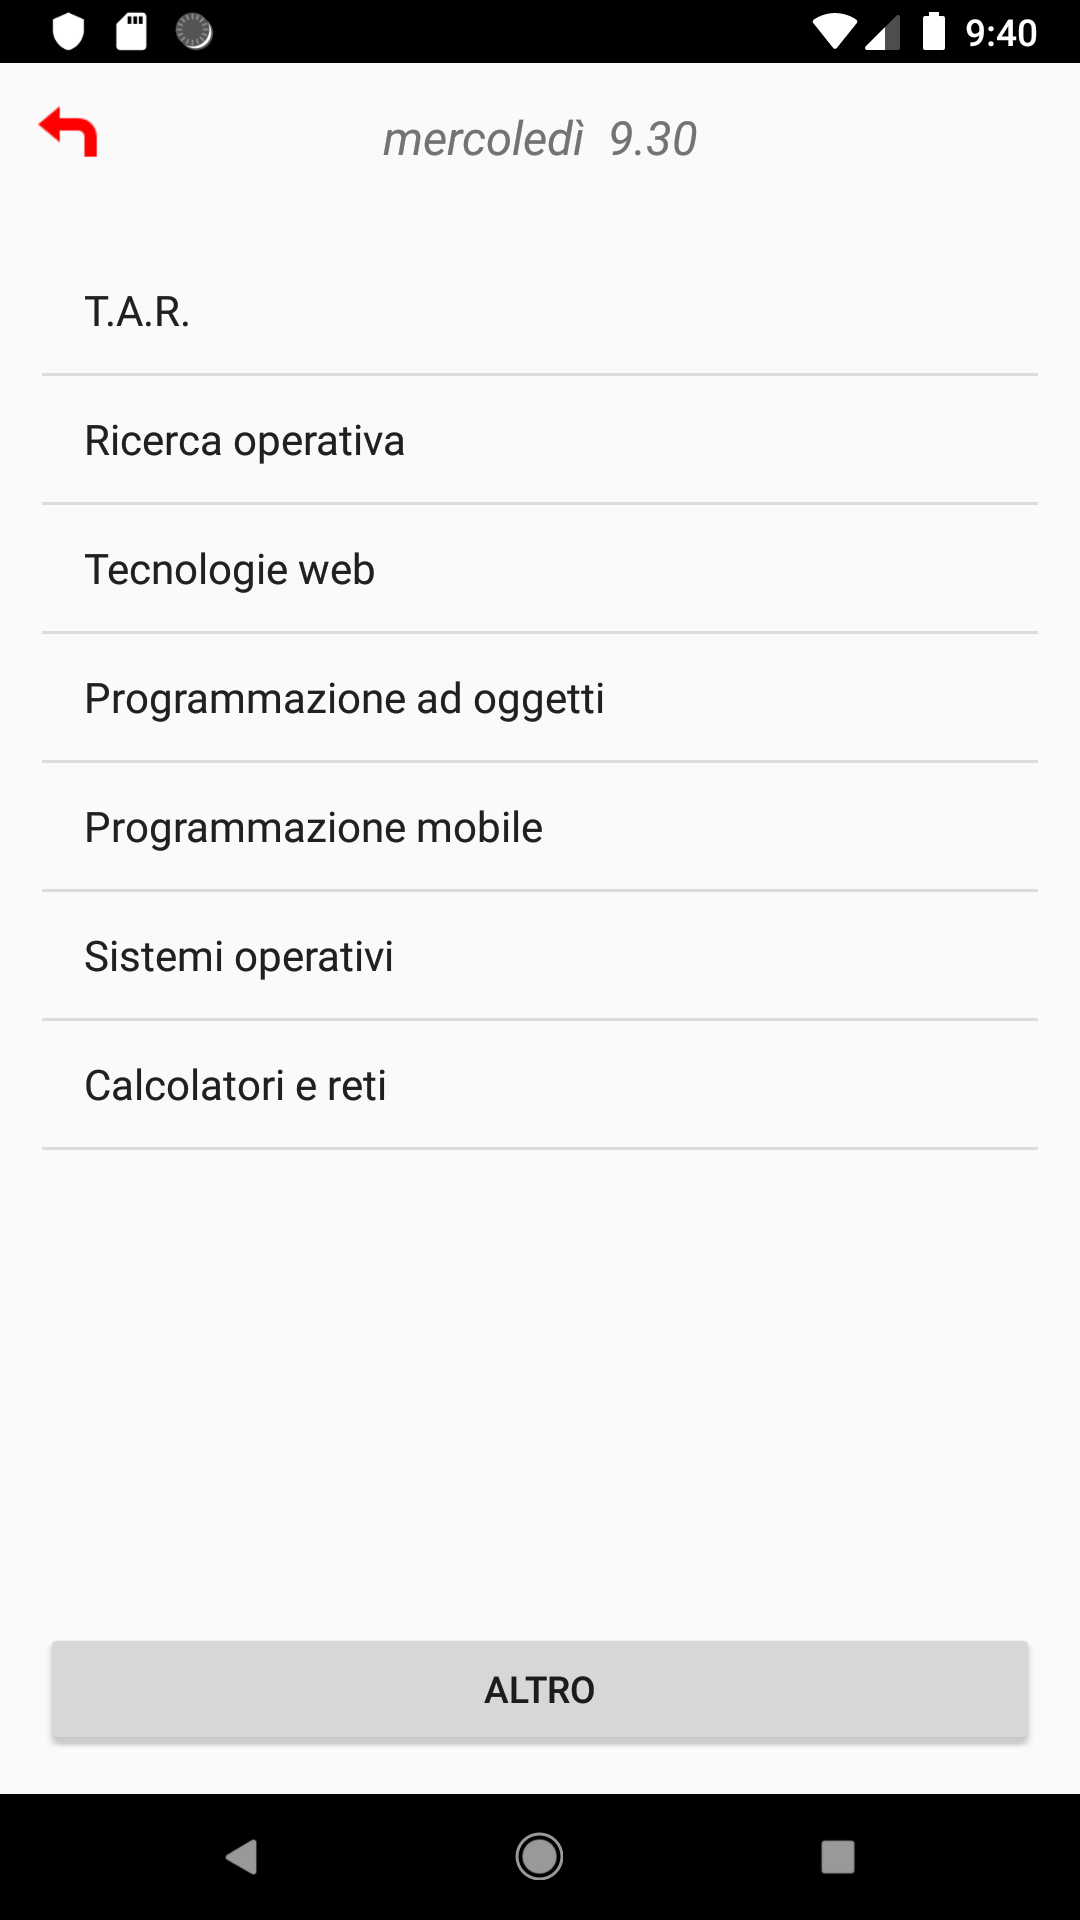
\includegraphics[width=.30\textwidth]{orario_scelta_materia}}\quad
	{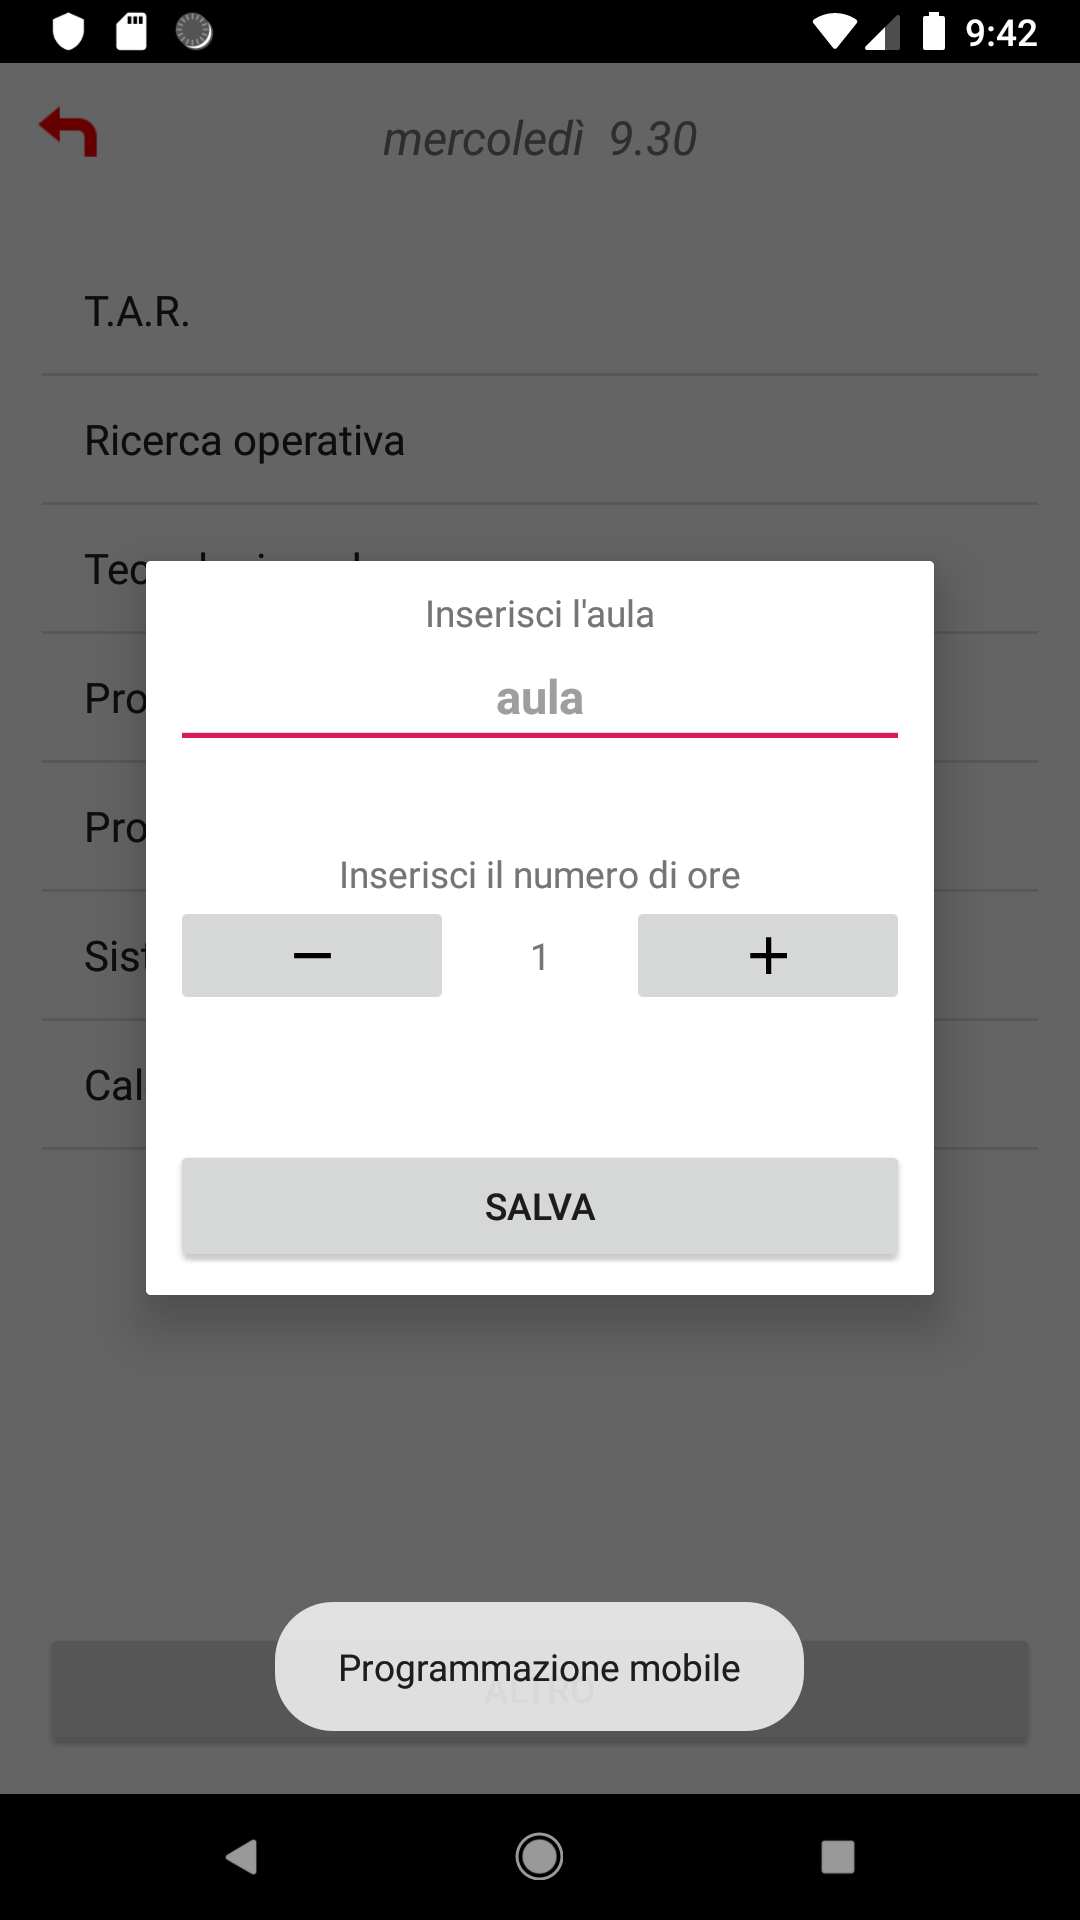
\includegraphics[width=.30\textwidth]{orario_inserimento}}
	\caption{\small Orario.}
\end{figure}

Salvata la materia nell'orario questa viene salvata nel database e inserita in una lista nella sezione \textbf{i miei appunti}.

\subsection{I miei appunti}
In questa sezione abbiamo accesso alla lista di tutte le materie salvate nel database. Abbiamo la possibilità di aggiungerne altre a piacimento o eliminarle inserendo il nome esatto della materia.

\begin{figure}[!h]
	\centering
	{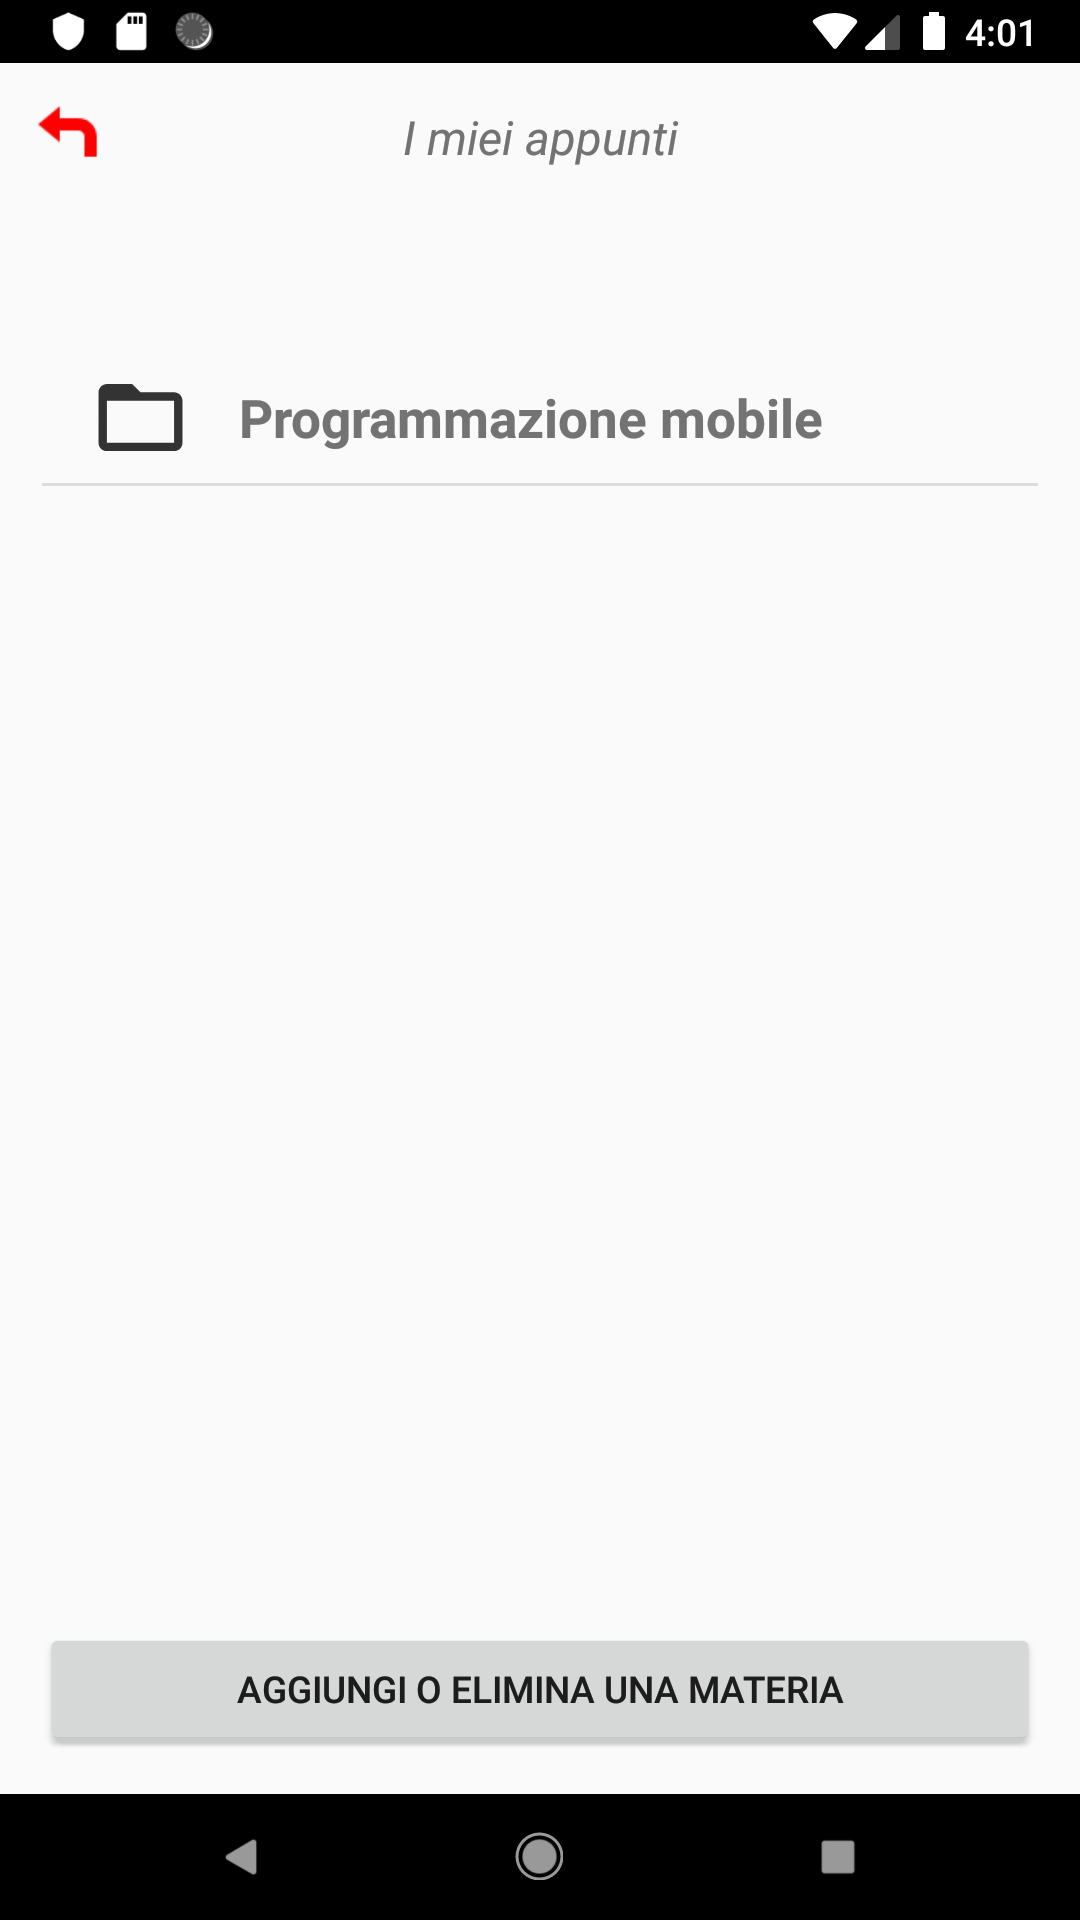
\includegraphics[width=.30\textwidth]{miei_appunti_lista_materie}} \quad
	{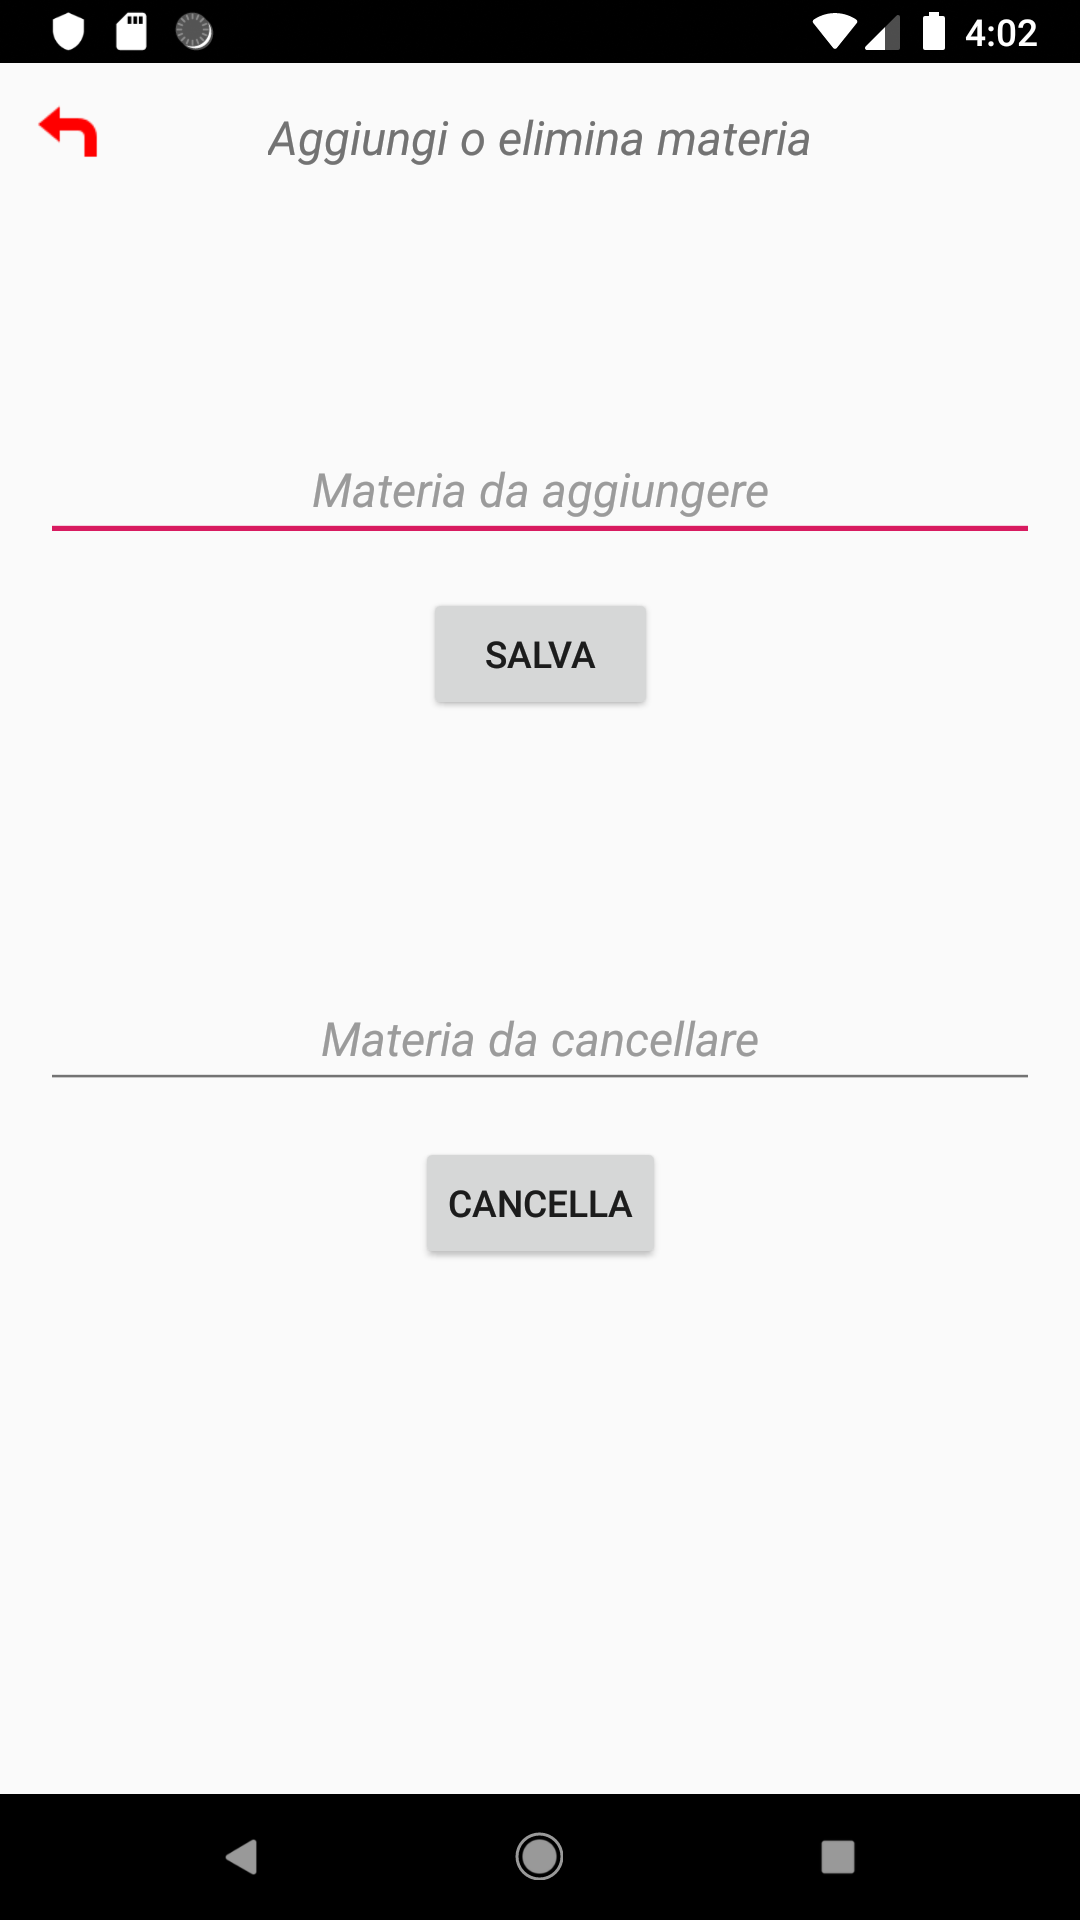
\includegraphics[width=.30\textwidth]{miei_appunti_aggiungi_materia}} \quad
	{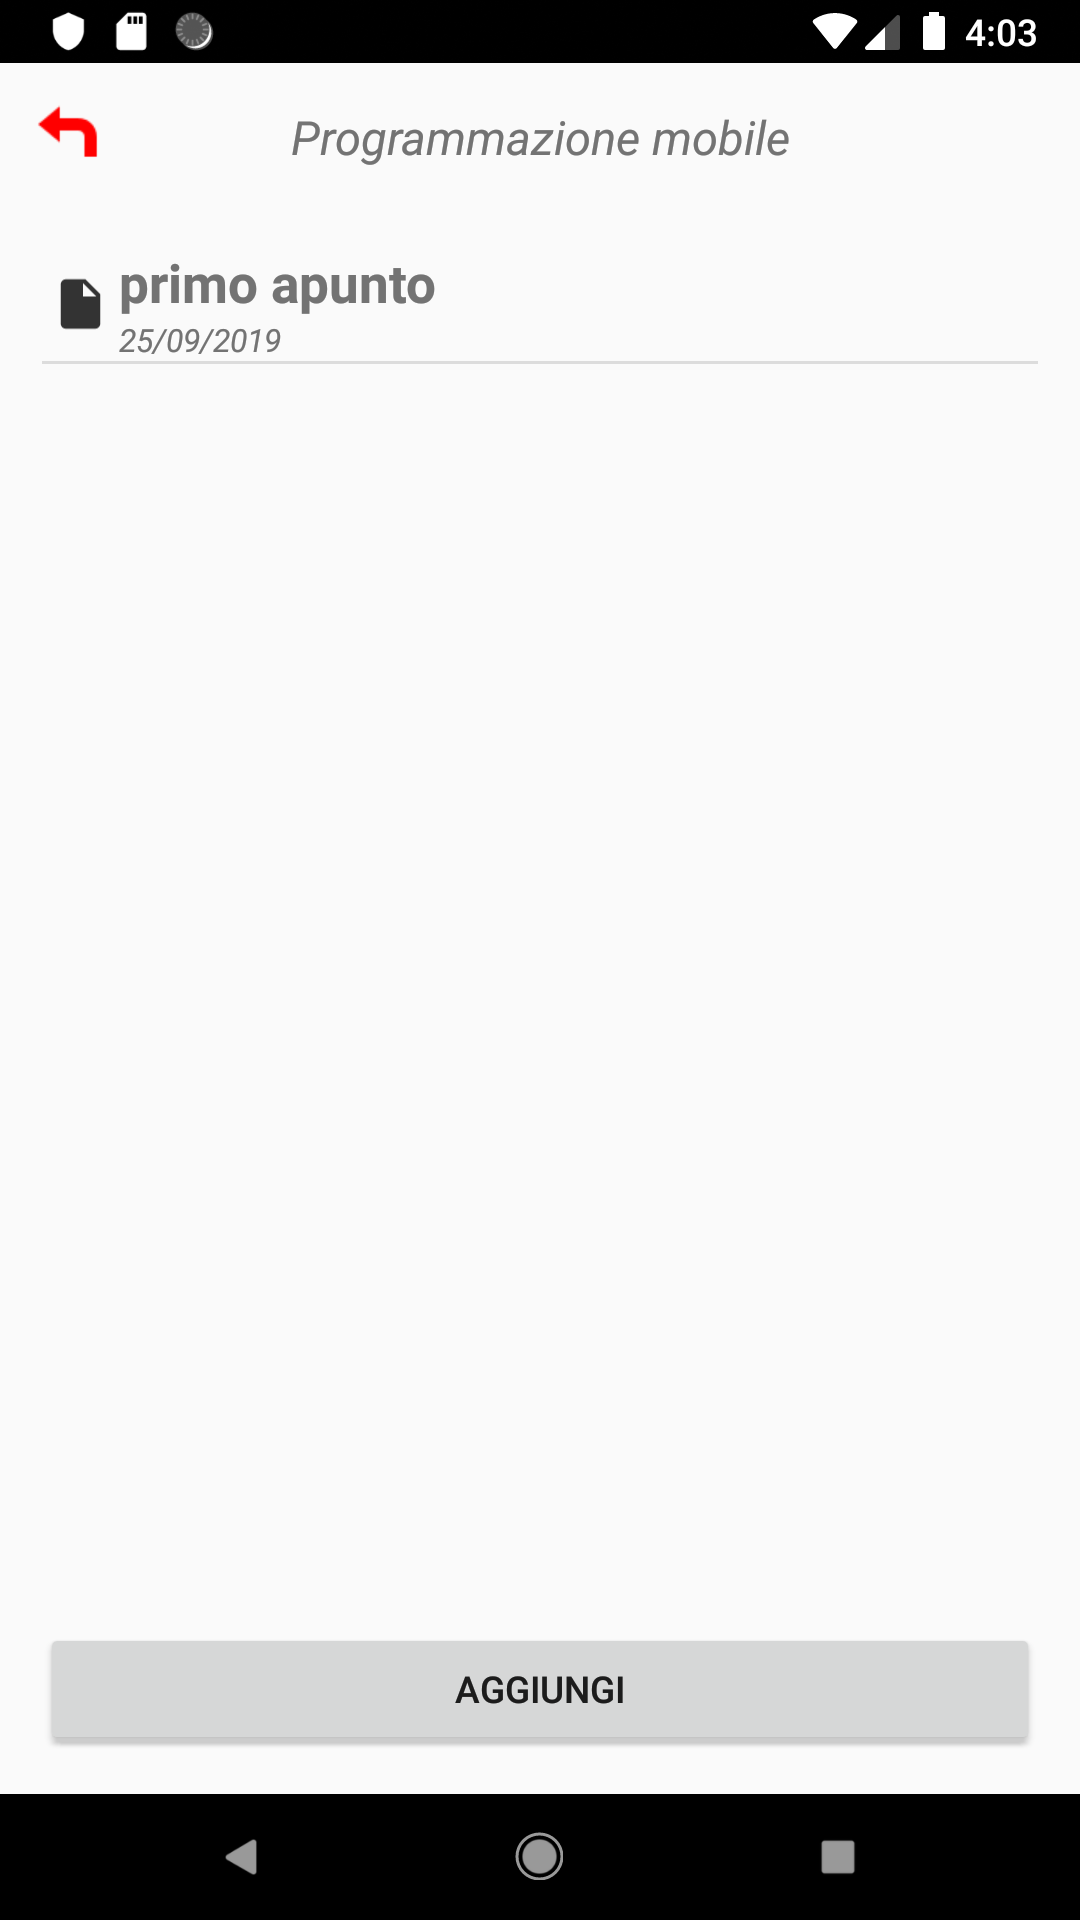
\includegraphics[width=.30\textwidth]{miei_appunti_lista_appunti}}
	\caption{\small Scegli aggiungi o elimina una materia e scegli un appunto.}
\end{figure}

Scelta la materia accediamo ad una seconda lista contenente tutti gli appunti relativi ad essa; ogni elemento della lsita contiene titolo e data relativi ad ogni appunto.
Da questa lista possiamo accedere e visualizzare l'annotazione vera e propria.

Gli appunti possono essere aggiunti con il bottone \textbf{"aggiungi"}, qui inseriremo titolo data e annotazione che vogliamo salvare; da questa schermata, inserendo la spunta nel campo \textbf{"Condividi"}, possono essere condivisi direttamente gli appunti con gli altri utenti.

Per eliminare un appunto basta tenere premuto l'elemento da eliminare, verrà attivata una finestra di dialogo da cui è possibile confermare la cancellazione.

\begin{figure}[!h]
	\centering
	{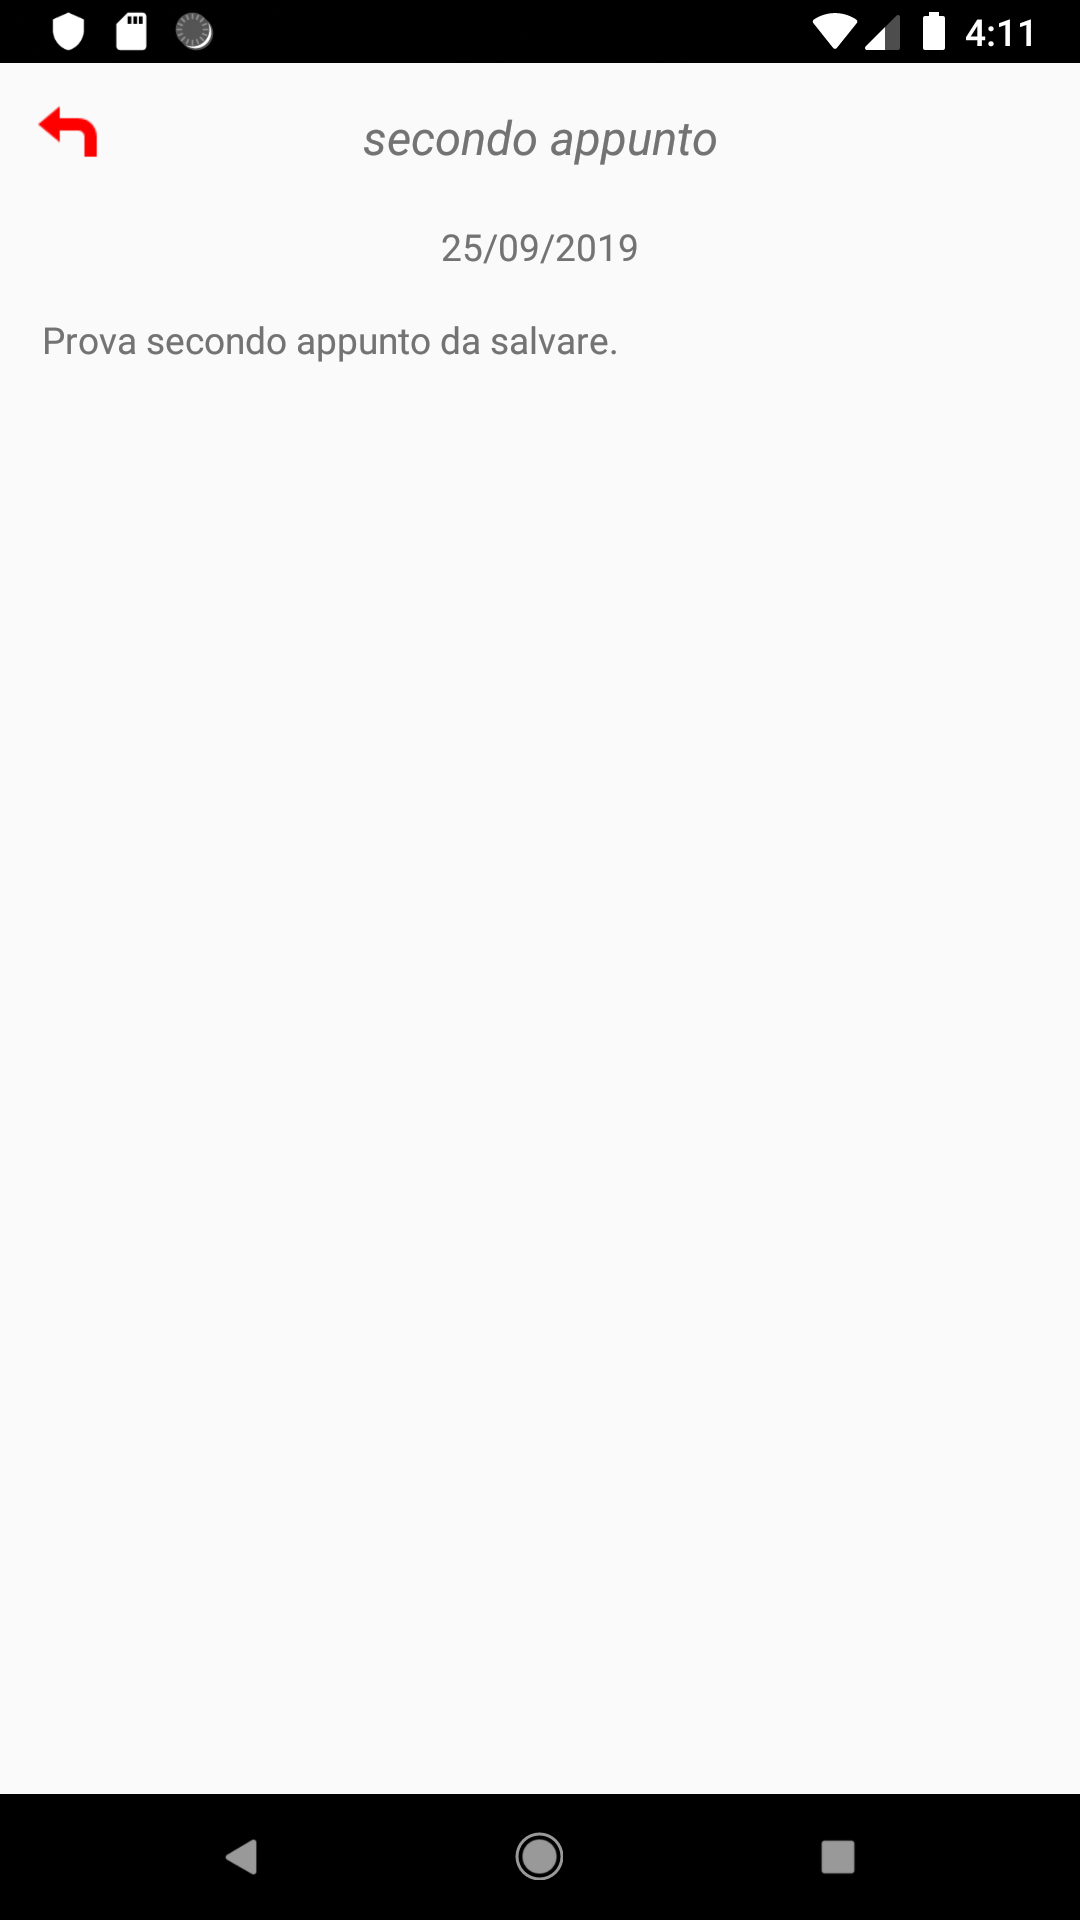
\includegraphics[width=.30\textwidth]{miei_appunti_vedi_appunto}} \quad
	{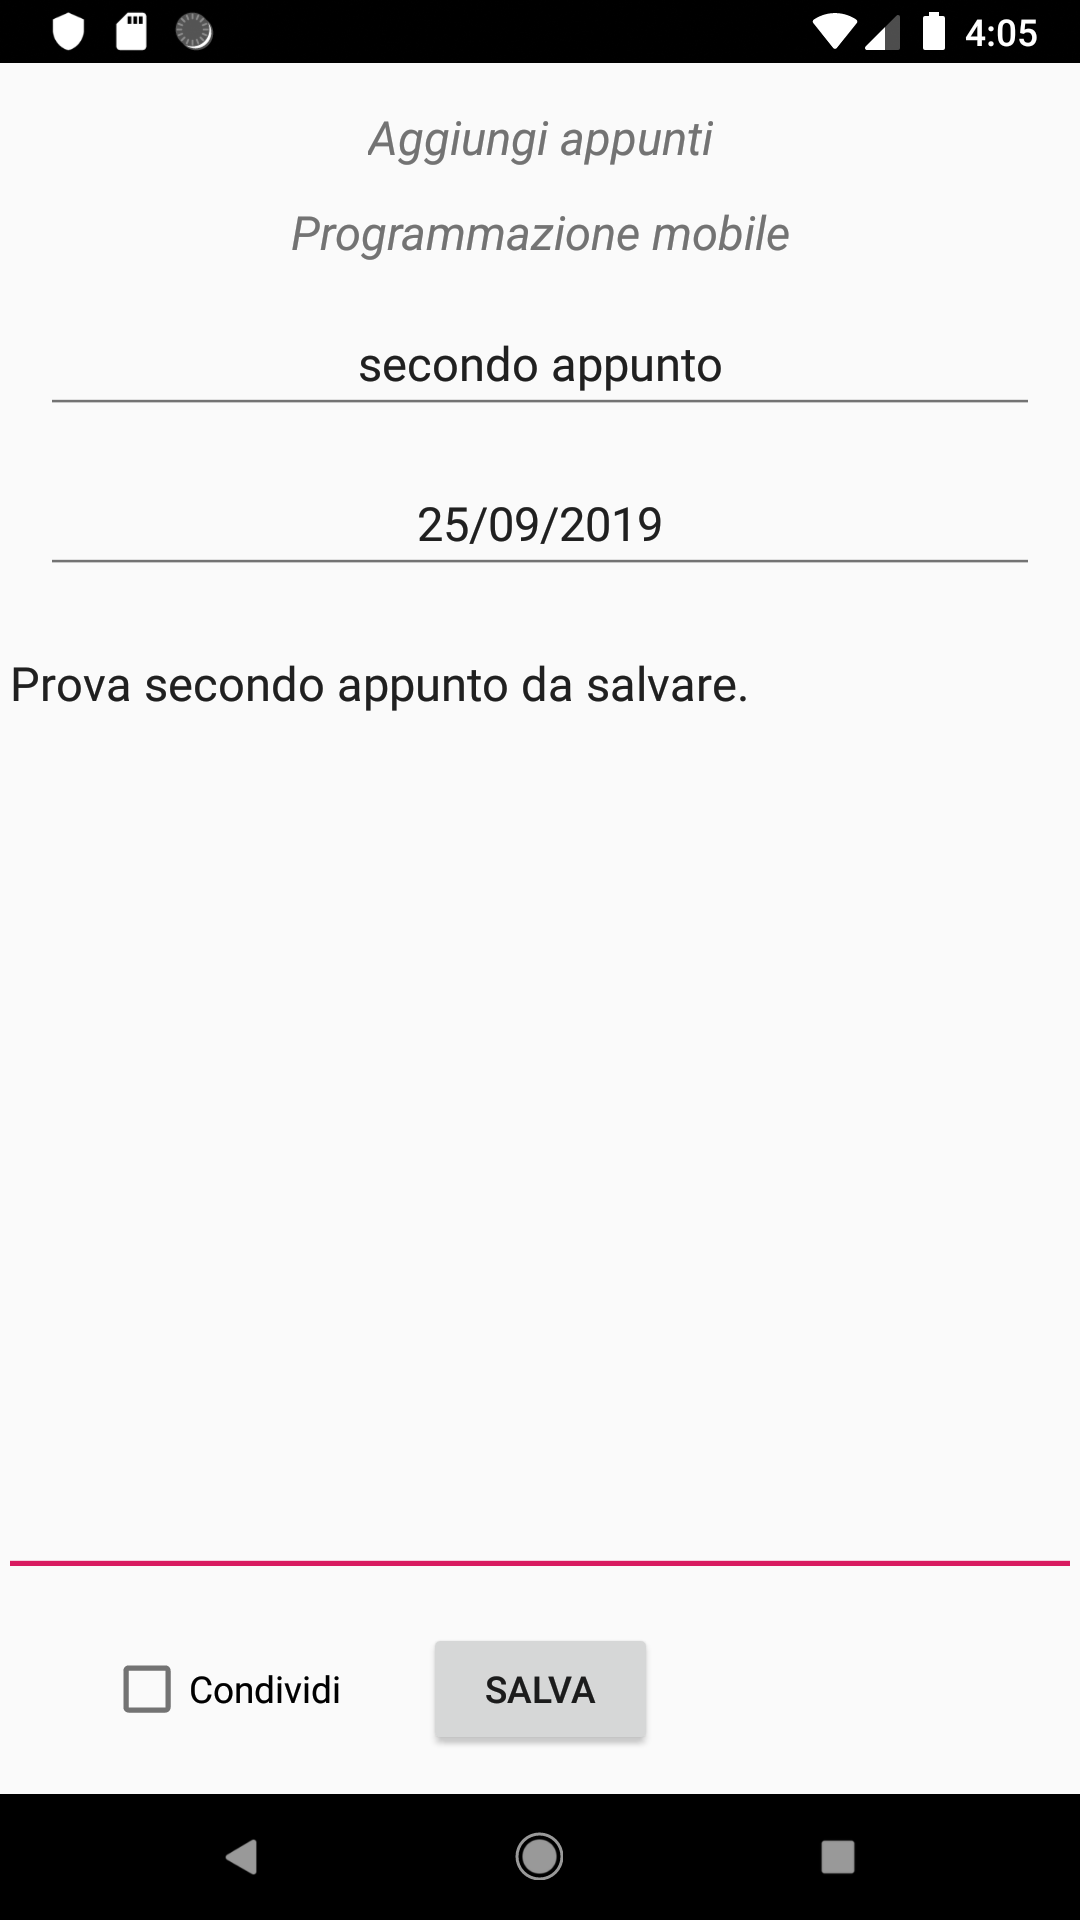
\includegraphics[width=.30\textwidth]{miei_appunti_aggiungi_appunto}} \quad
	{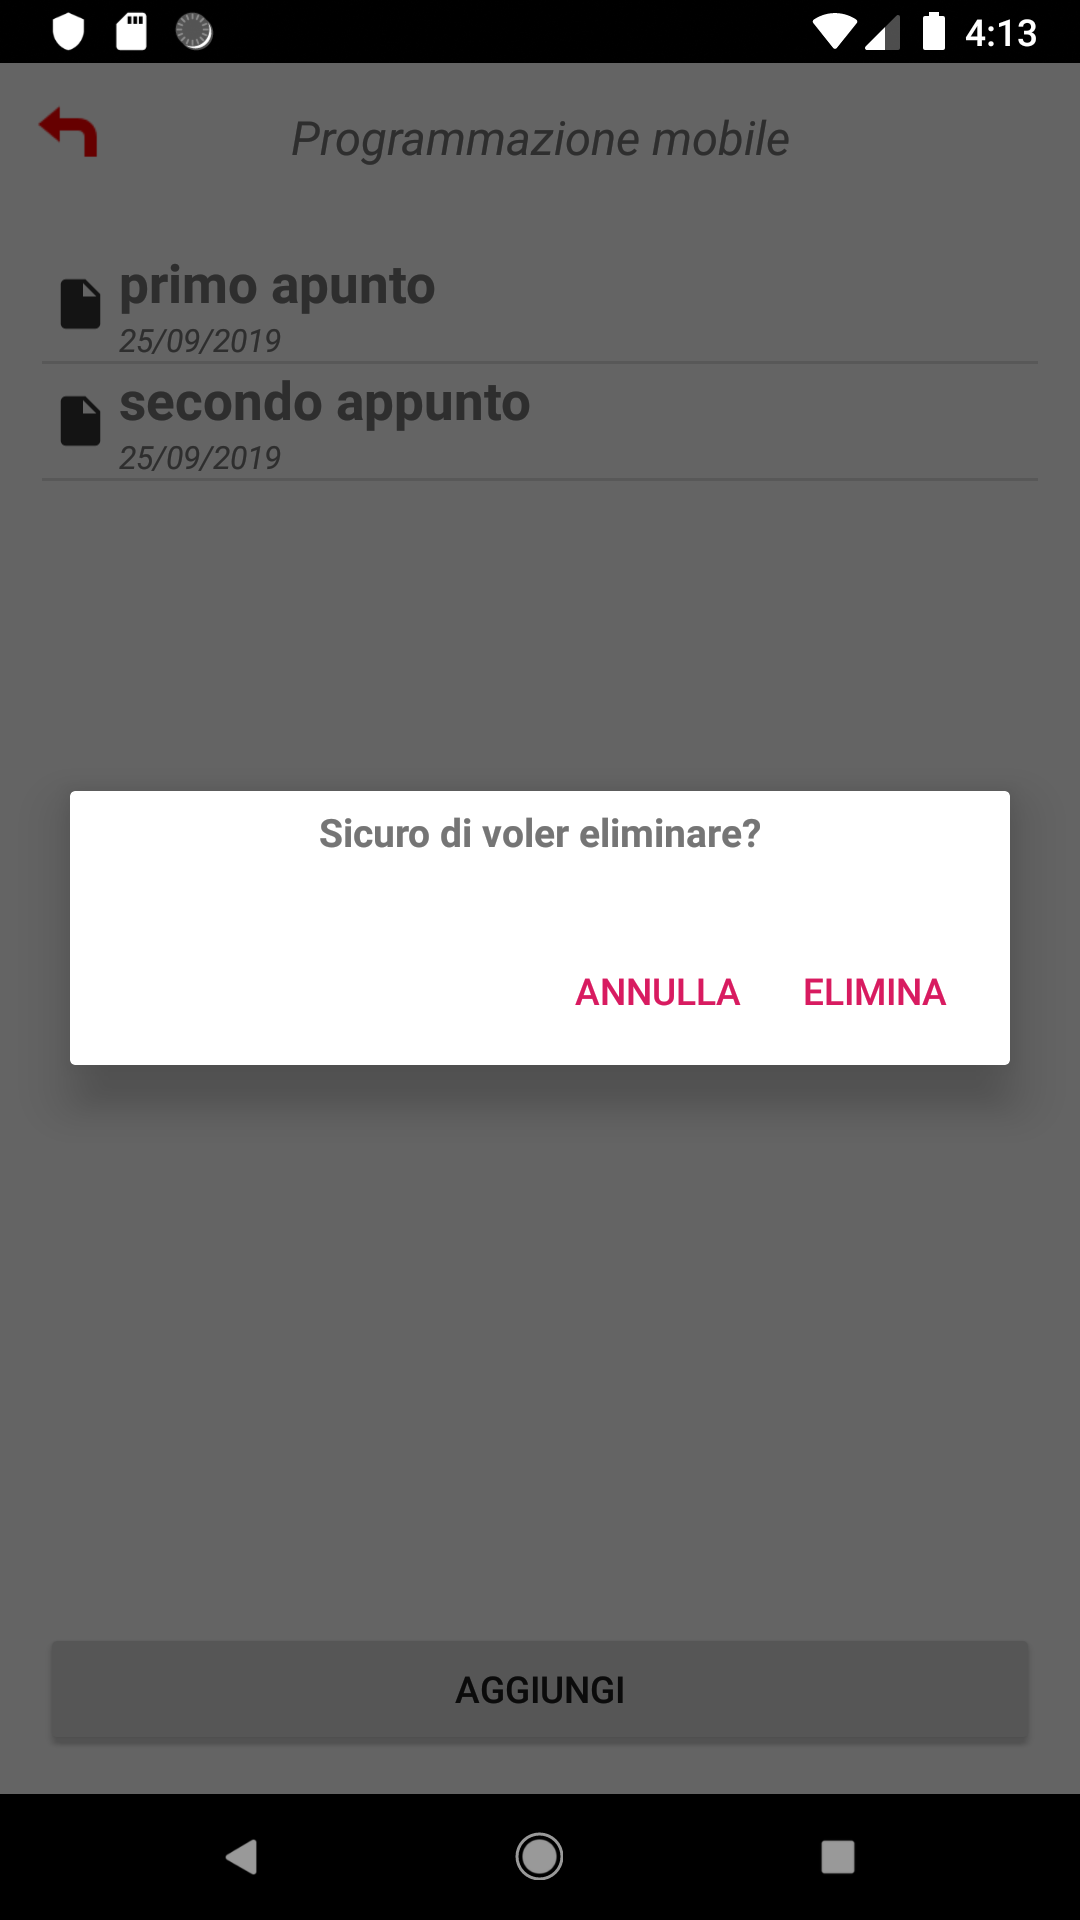
\includegraphics[width=.30\textwidth]{miei_appunti_elimina_appunto}}
	\caption{\small Visualizza, aggiungi o elimina un appunto.}
\end{figure}

\subsection{Appunti condivisi}
Nella sezione appunti condivisi possiamo scegliere una delle materie predefinite in lista per visualizzare gli appunti che sono stati condivisi ed eventualmente visualizzarli o scaricarli.

\begin{figure}[!h]
	\centering
	{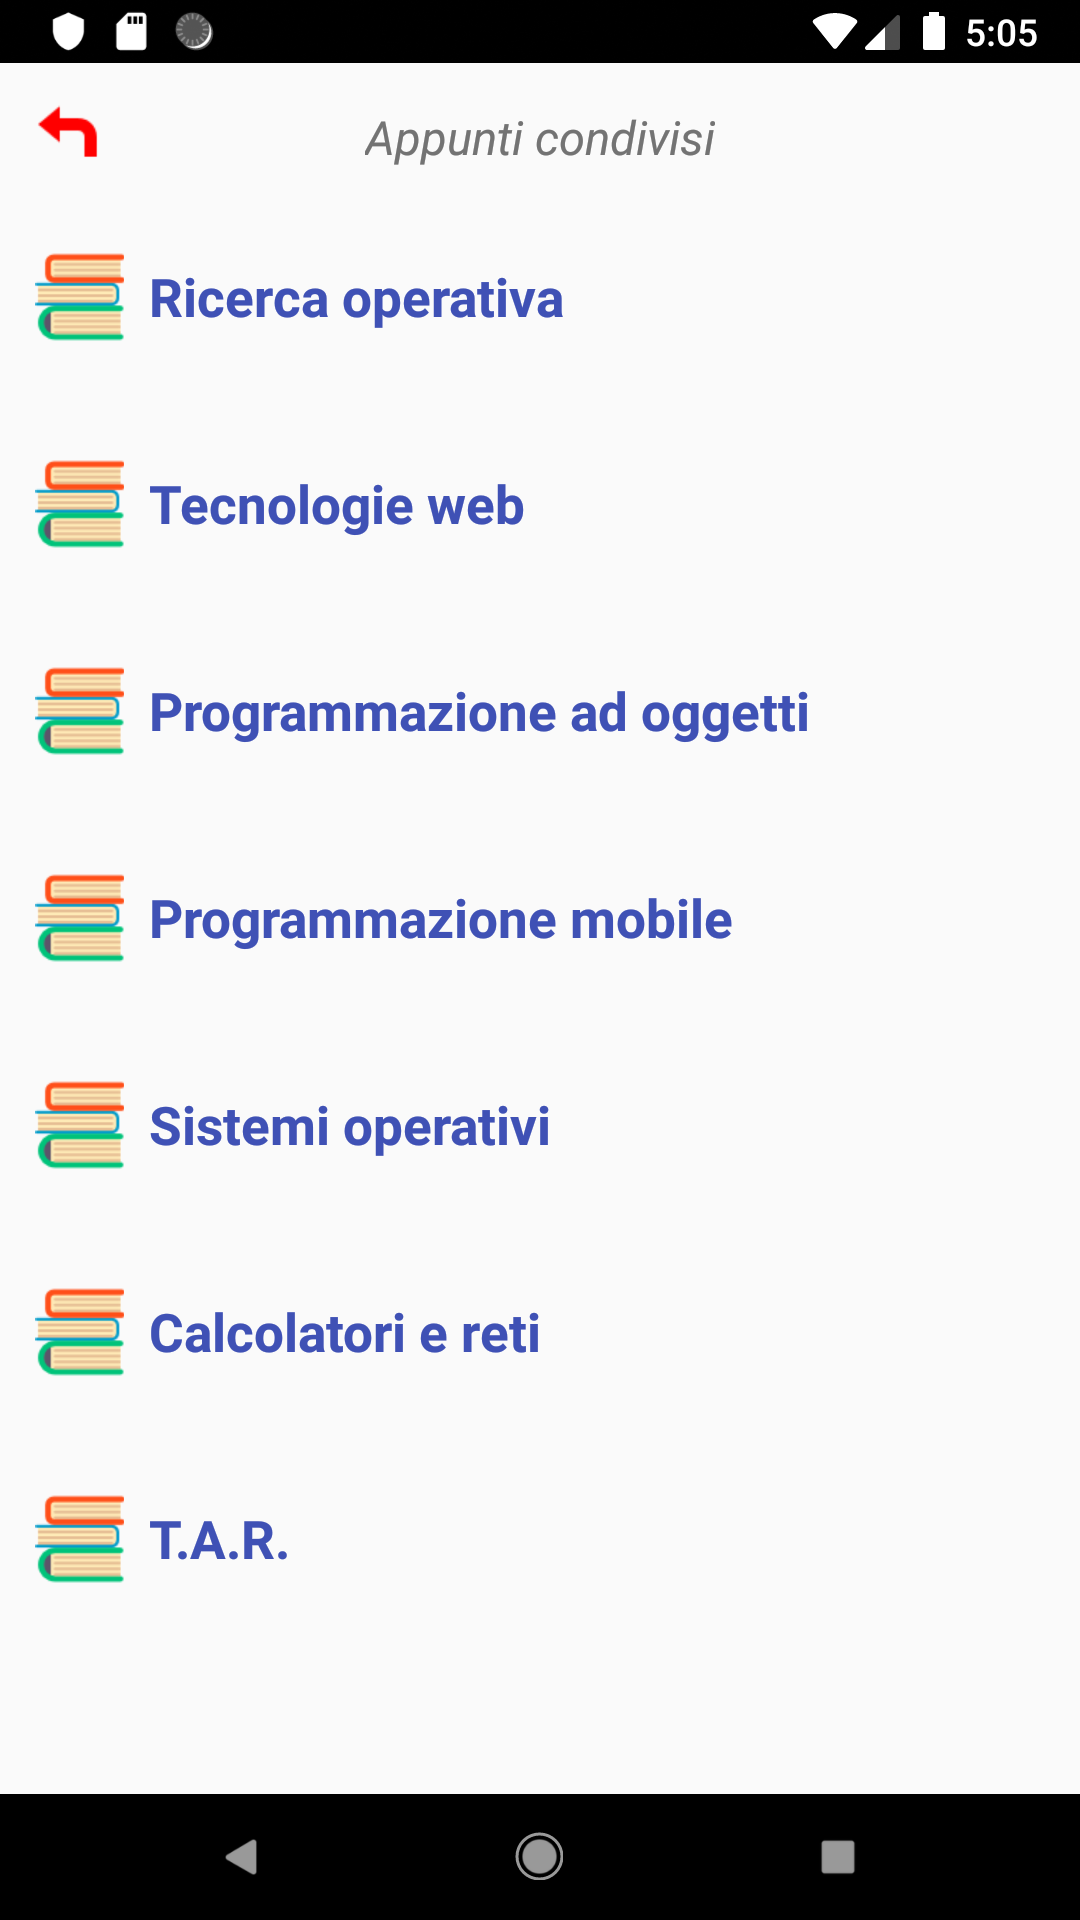
\includegraphics[width=.30\textwidth]{appunti_condivisi_lista_materie}} \quad
	{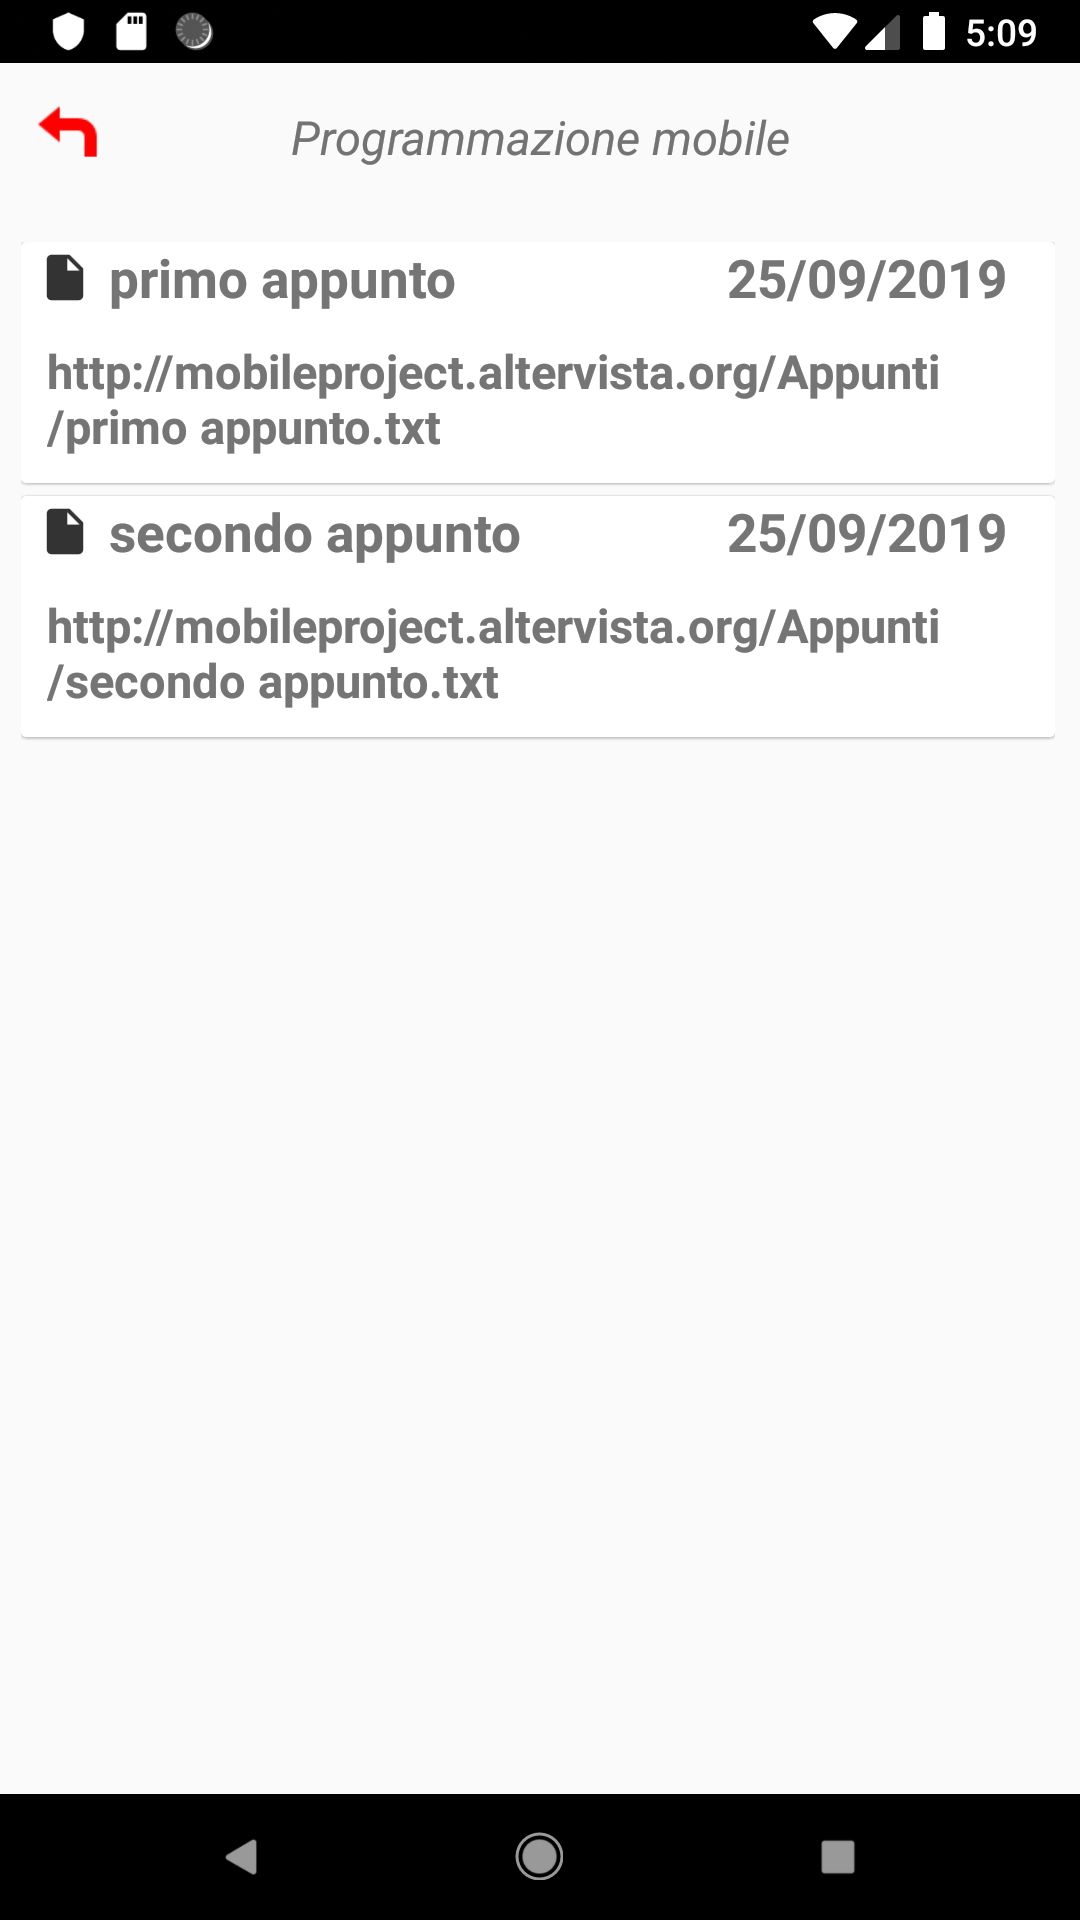
\includegraphics[width=.30\textwidth]{appunti_condivisi_lista_appunti}} \quad
	{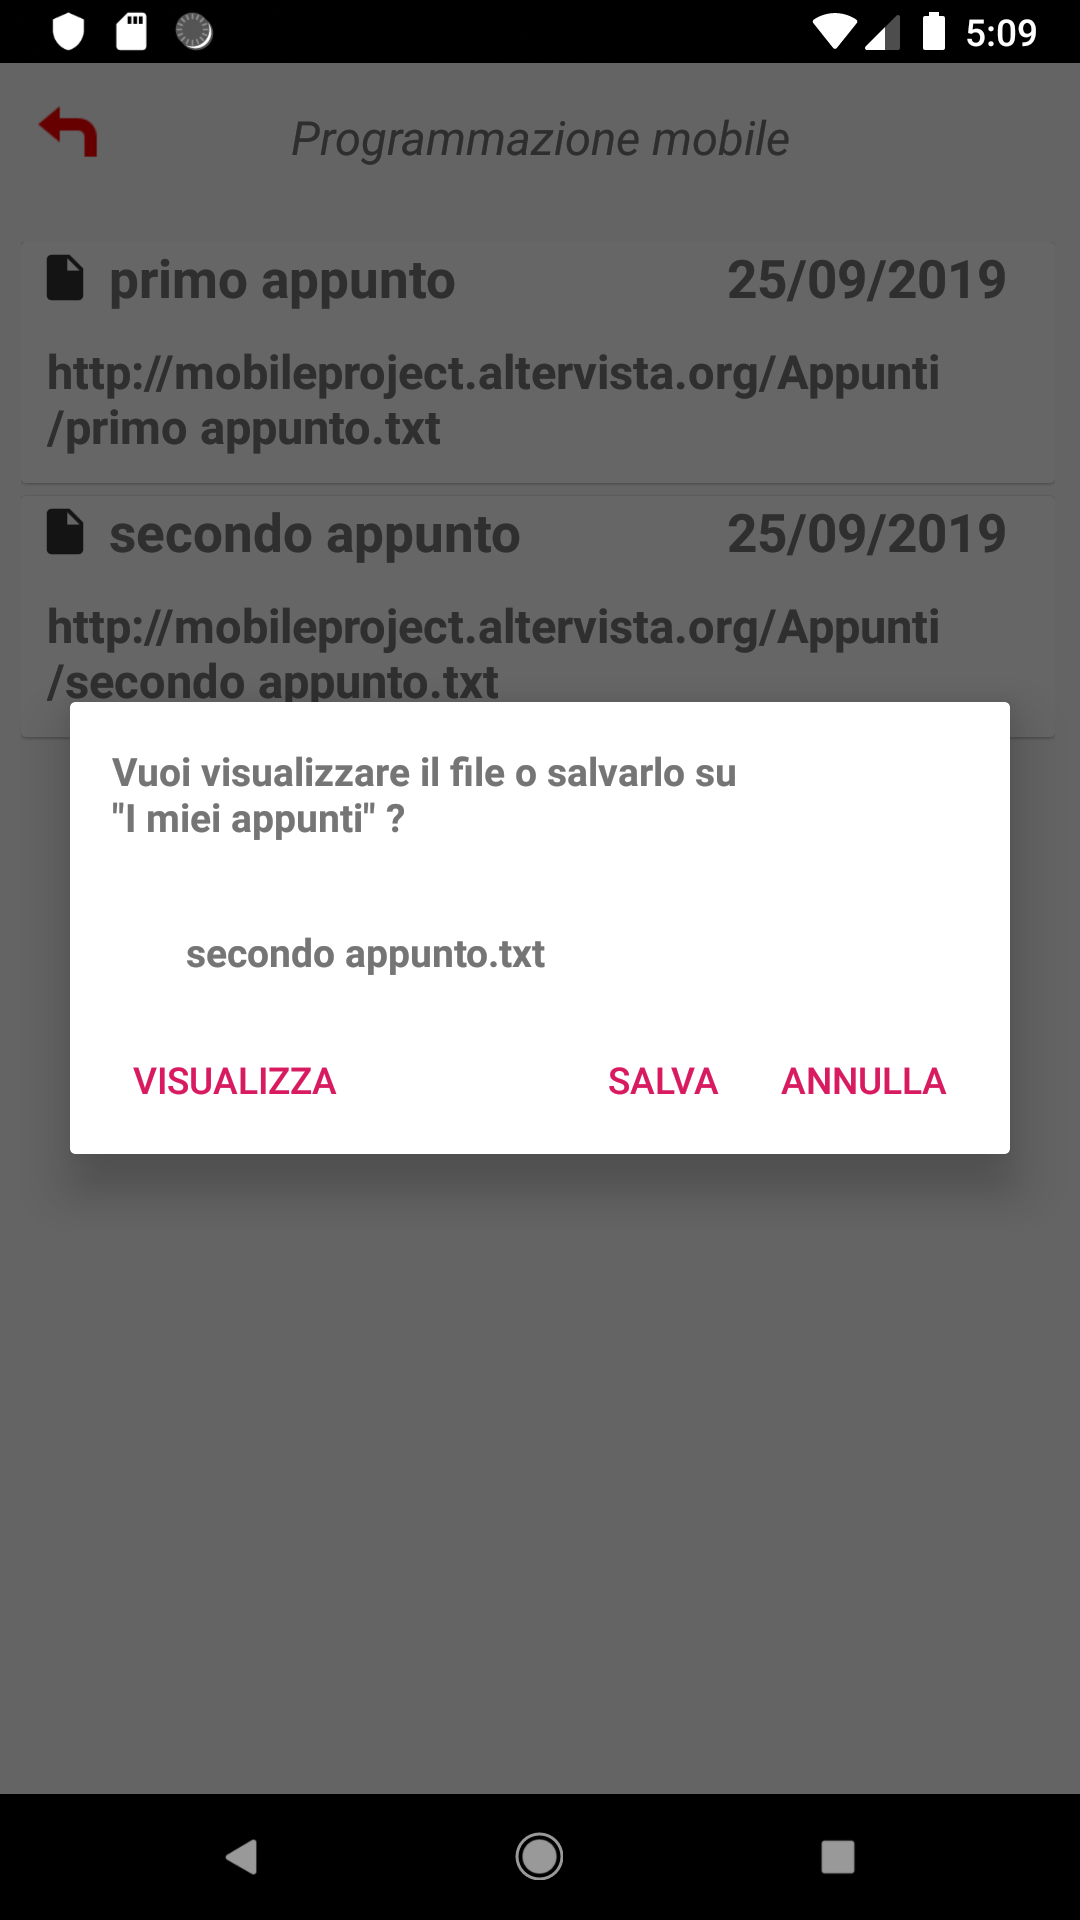
\includegraphics[width=.30\textwidth]{appunti_condivisi_scegli_azione}}
	\caption{\small Appunti condivisi, scegli la materia, scegli l'appunto, visualizza o scarica.}
\end{figure}

\subsection{Impostazioni}
Dalle impostazioni possiamo banalmente modificare \textbf{username}, \textbf{password} e leggere informazioni \textbf{about us}.

\begin{figure}[!h]
	\centering
	{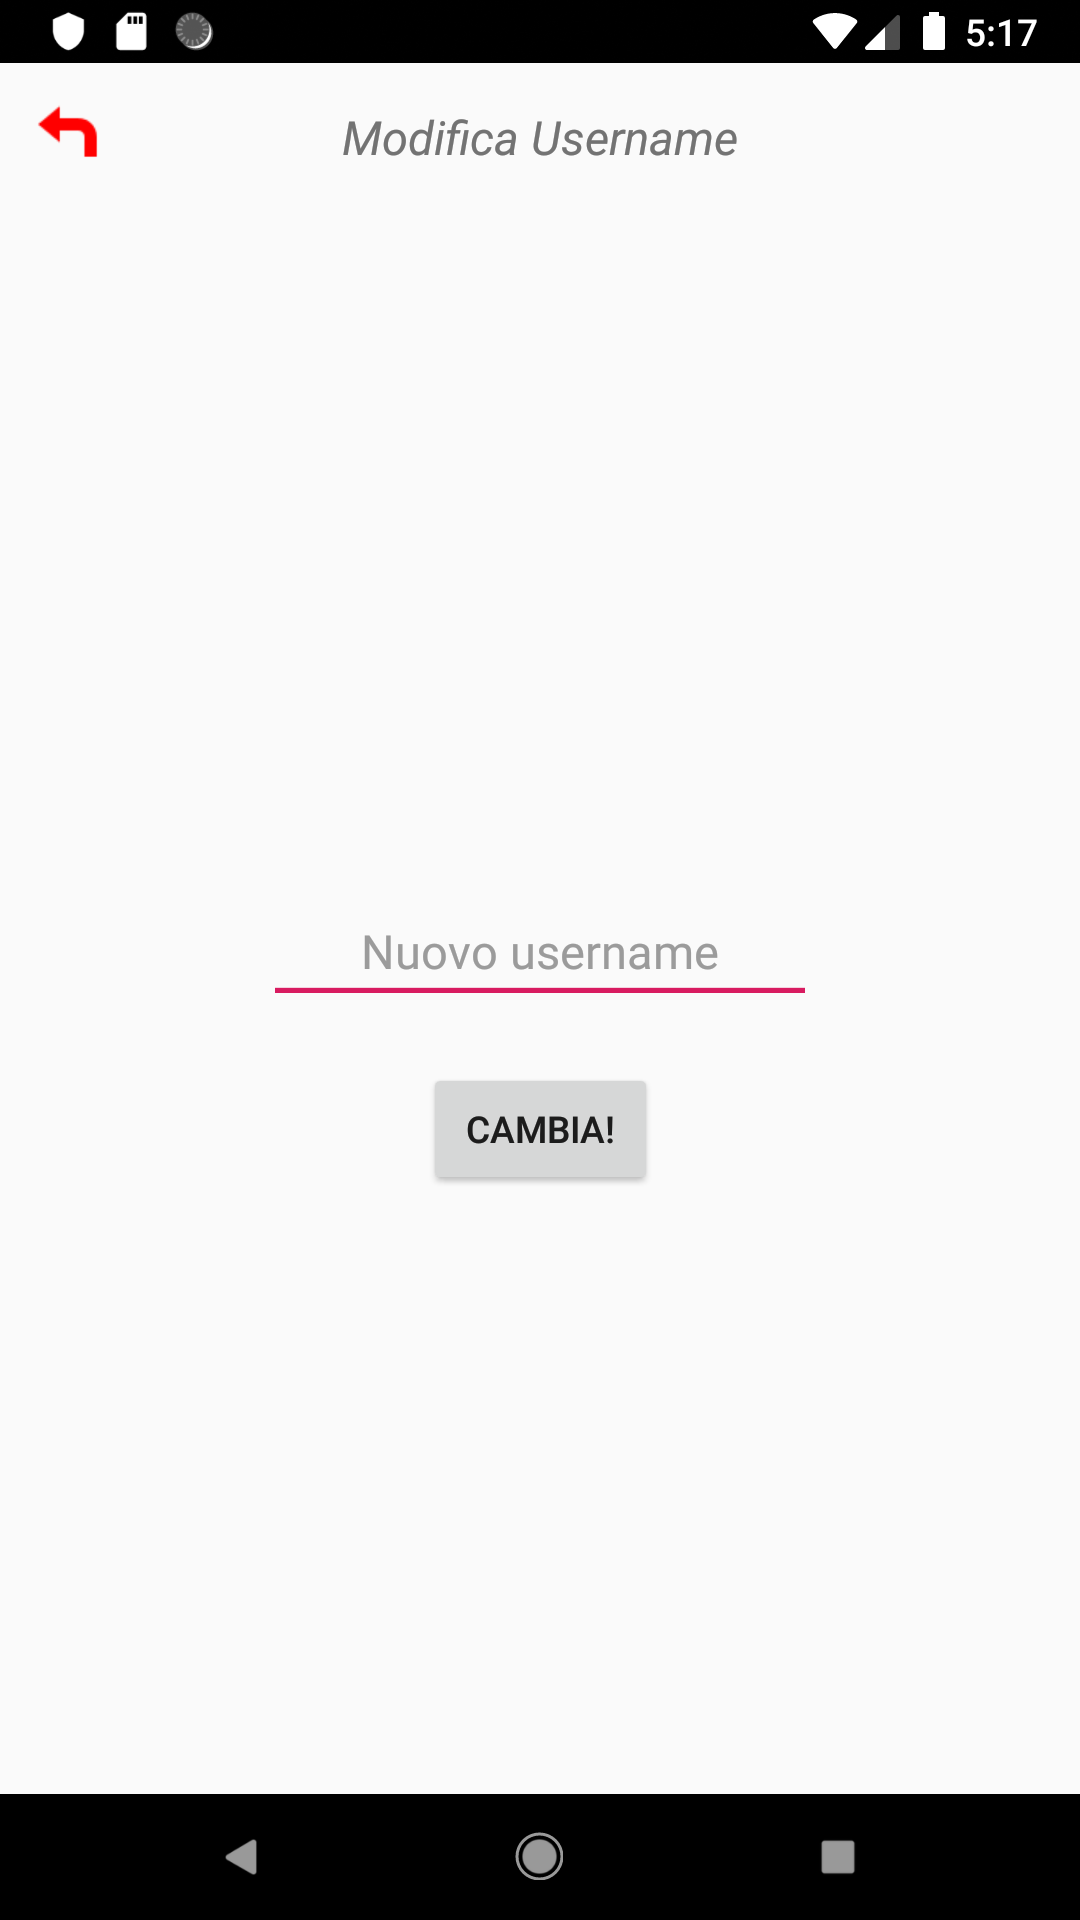
\includegraphics[width=.30\textwidth]{impostazioni_username}} \quad
	{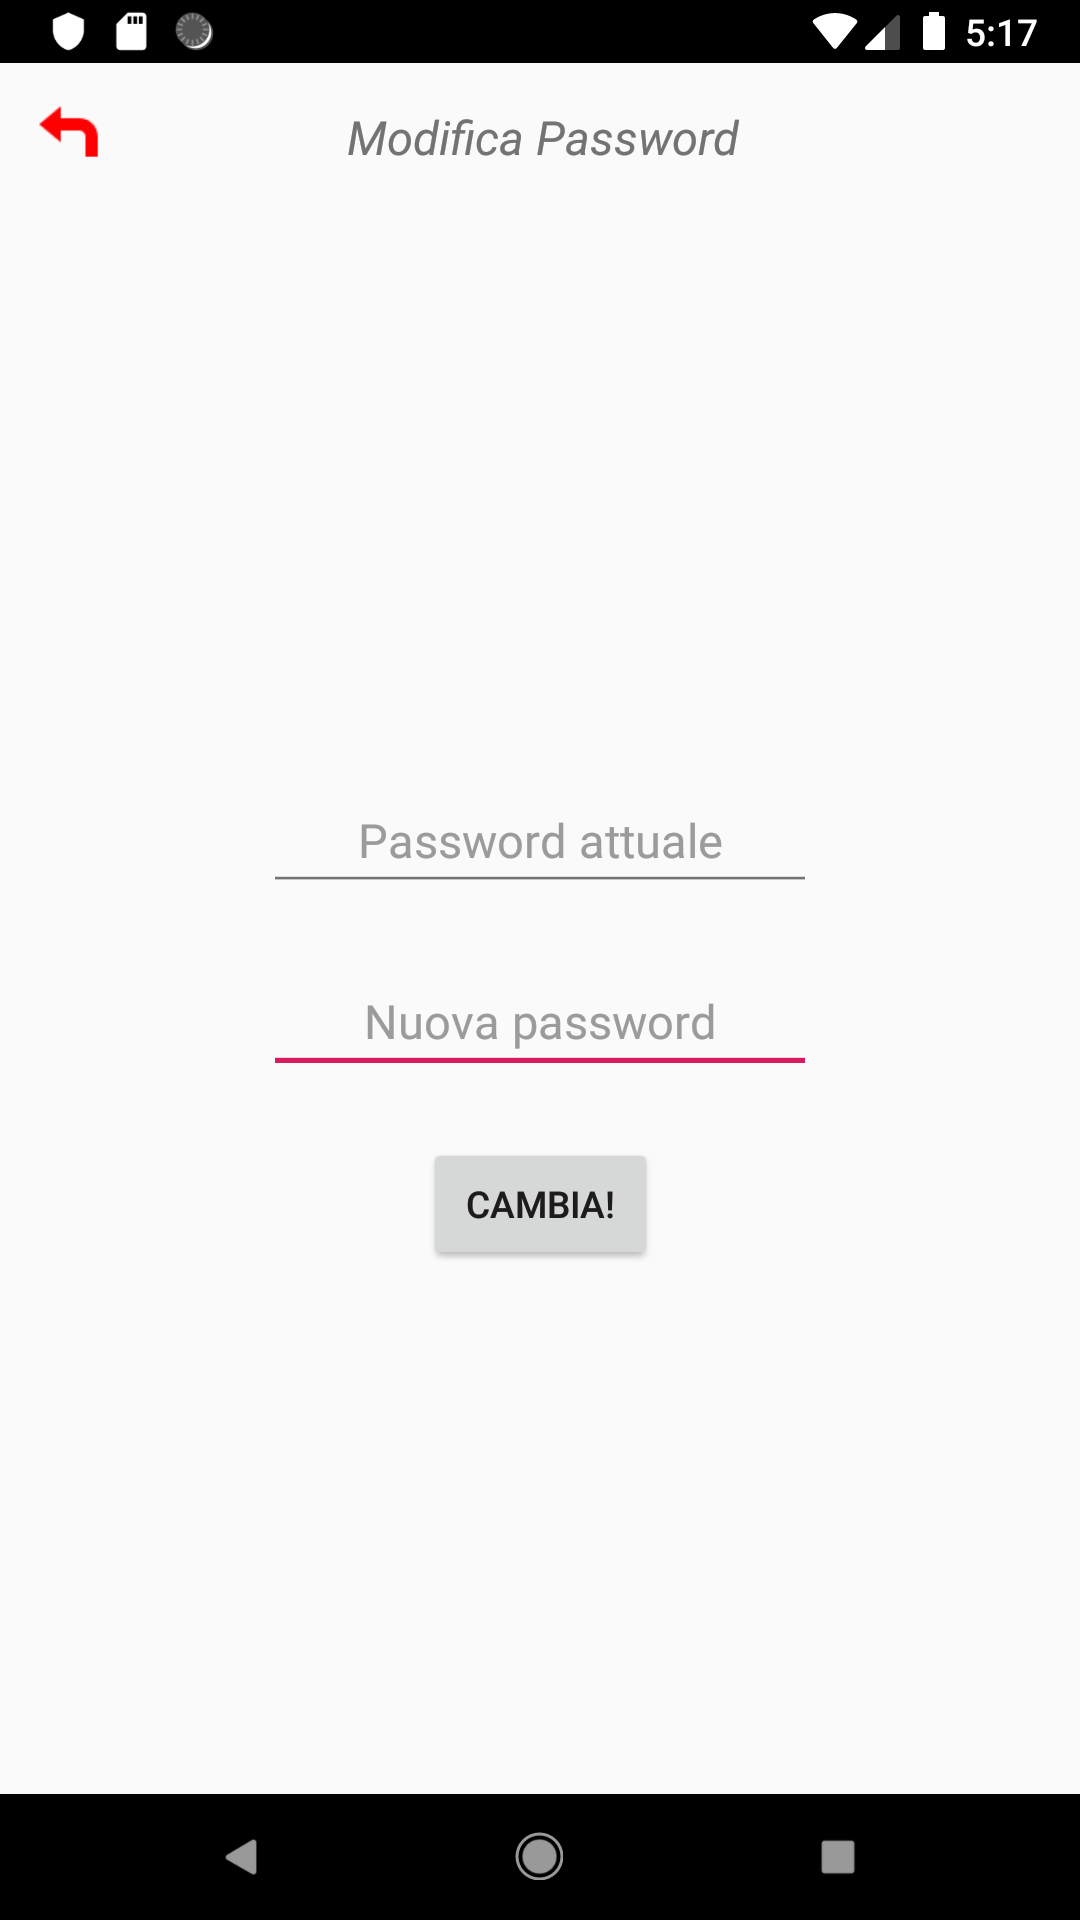
\includegraphics[width=.30\textwidth]{impostazioni_password}} \quad
	{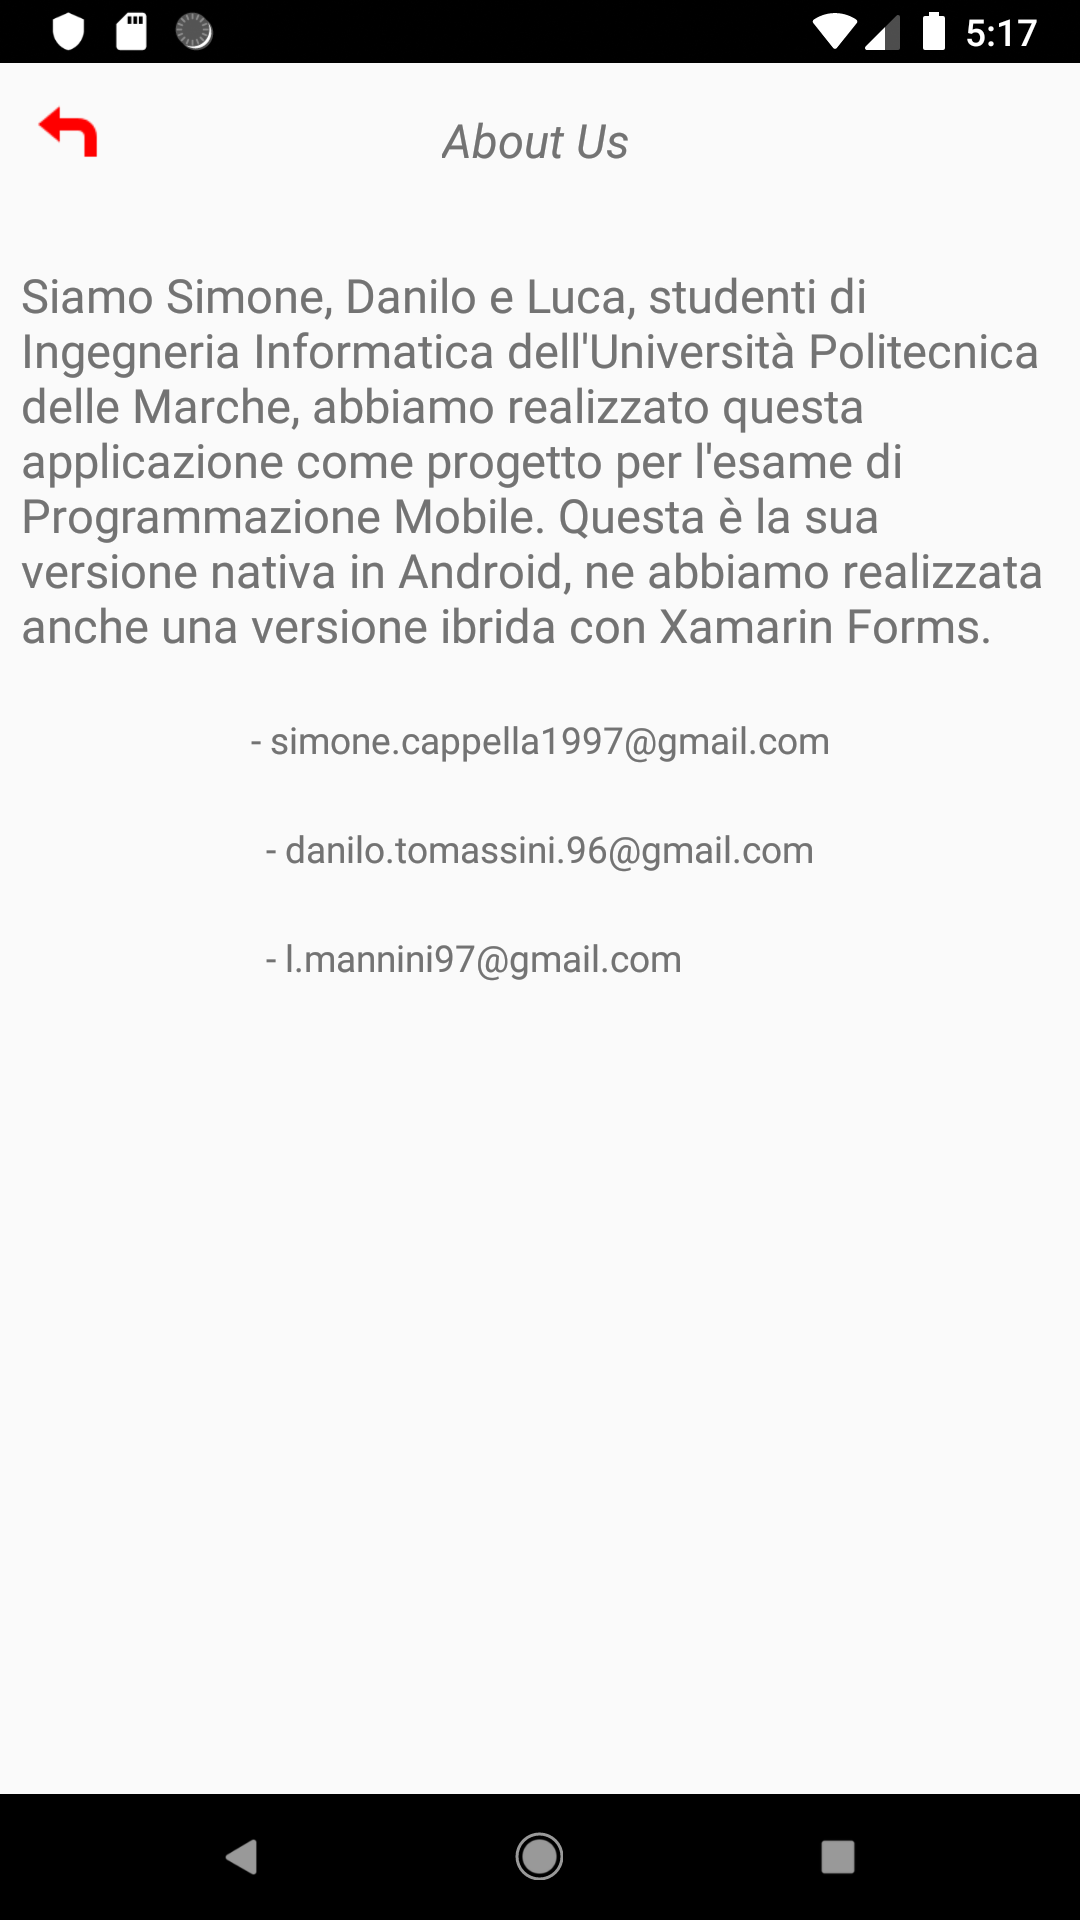
\includegraphics[width=.30\textwidth]{impostazioni_about_us}}
	\caption{\small Azioni eseguibili nelle impostazioni.}
\end{figure}


















































\end{document}